\documentclass[a4paper,12pt,twoside]{memoir}

% Castellano
\usepackage[spanish,es-tabla]{babel}
\selectlanguage{spanish}
\usepackage[utf8]{inputenc}
\usepackage[T1]{fontenc}
\usepackage{lmodern} % scalable font
\usepackage{microtype}
\usepackage{placeins}
\usepackage{csquotes}
\usepackage{lscape} 
\usepackage[table,xcdraw]{xcolor}
\usepackage{graphicx}
\usepackage{float} %required for the placement specifier H

\usepackage{makecell}

\renewcommand\theadalign{bc}
\renewcommand\theadfont{\bfseries}
\renewcommand\theadgape{\Gape[4pt]}
\renewcommand\cellgape{\Gape[4pt]}

% Landscape
\usepackage{pdflscape}

% Mathematic font
\usepackage{amsfonts}

\RequirePackage{booktabs}
\RequirePackage[table]{xcolor}
\RequirePackage{xtab}
\RequirePackage{multirow}

% Multi-page tables using
\nouppercaseheads
\usepackage{longtable}
\usepackage{tabularx}

% Cell with line break (e.g. \specialcell{Foo\\bar})
\newcommand{\specialcell}[2][c]{%
  \begin{tabular}[#1]{@{}l@{}}#2\end{tabular}}

% Links
\PassOptionsToPackage{hyphens}{url}\usepackage[colorlinks]{hyperref}
\hypersetup{
	allcolors = {blue}
}

% Ecuaciones
\usepackage{amsmath}

% Rutas de fichero / paquete
\newcommand{\ruta}[1]{{\sffamily #1}}

% Párrafos
\nonzeroparskip

% Huérfanas y viudas
\widowpenalty100000
\clubpenalty100000

% Evitar solapes en el header
%\nouppercaseheads

% Imagenes
\usepackage{graphicx}
\newcommand{\imagen}[2]{
	\begin{figure}[!h]
		\centering
		\includegraphics[width=0.9\textwidth]{#1}
		\caption{#2}\label{fig:#1}
	\end{figure}
	\FloatBarrier
}

\newcommand{\imagenflotante}[2]{
	\begin{figure}%[!h]
		\centering
		\includegraphics[width=0.9\textwidth]{#1}
		\caption{#2}\label{fig:#1}
	\end{figure}
}

\usepackage{listings}
\usepackage{xcolor}

\colorlet{punct}{red!60!black}
\definecolor{background}{HTML}{EEEEEE}
\definecolor{delim}{RGB}{20,105,176}
\colorlet{numb}{magenta!60!black}

\lstdefinelanguage{json}{
    basicstyle=\normalfont\ttfamily,
    numbers=left,
    numberstyle=\scriptsize,
    stepnumber=1,
    numbersep=8pt,
    showstringspaces=false,
    breaklines=true,
    frame=lines,
    backgroundcolor=\color{background},
    literate=
     *{0}{{{\color{numb}0}}}{1}
      {1}{{{\color{numb}1}}}{1}
      {2}{{{\color{numb}2}}}{1}
      {3}{{{\color{numb}3}}}{1}
      {4}{{{\color{numb}4}}}{1}
      {5}{{{\color{numb}5}}}{1}
      {6}{{{\color{numb}6}}}{1}
      {7}{{{\color{numb}7}}}{1}
      {8}{{{\color{numb}8}}}{1}
      {9}{{{\color{numb}9}}}{1}
      {:}{{{\color{punct}{:}}}}{1}
      {,}{{{\color{punct}{,}}}}{1}
      {\{}{{{\color{delim}{\{}}}}{1}
      {\}}{{{\color{delim}{\}}}}}{1}
      {[}{{{\color{delim}{[}}}}{1}
      {]}{{{\color{delim}{]}}}}{1},
}
\definecolor{maroon}{cmyk}{0, 0.87, 0.68, 0.32}
\definecolor{halfgray}{gray}{0.55}
\definecolor{ipython_frame}{RGB}{207, 207, 207}
\definecolor{ipython_bg}{RGB}{247, 247, 247}
\definecolor{ipython_red}{RGB}{186, 33, 33}
\definecolor{ipython_green}{RGB}{0, 128, 0}
\definecolor{ipython_cyan}{RGB}{64, 128, 128}
\definecolor{ipython_purple}{RGB}{170, 34, 255}

\lstdefinelanguage{python}{
    morekeywords={access,and,break,class,continue,def,del,elif,else,except,exec,finally,for,from,global,if,import,in,is,lambda,not,or,pass,print,raise,return,try,while},
    morekeywords=[2]{abs,all,any,basestring,bin,bool,bytearray,callable,chr,classmethod,cmp,compile,complex,delattr,dict,dir,divmod,enumerate,eval,execfile,file,filter,float,format,frozenset,getattr,globals,hasattr,hash,help,hex,id,input,int,isinstance,issubclass,iter,len,list,locals,long,map,max,memoryview,min,next,object,oct,open,ord,pow,property,range,raw_input,reduce,reload,repr,reversed,round,set,setattr,slice,sorted,staticmethod,str,sum,super,tuple,type,unichr,unicode,vars,xrange,zip,apply,buffer,coerce,intern},
    sensitive=true,
    morecomment=[l]\#,
    morestring=[b]',
    morestring=[b]",
    morestring=[s]{'''}{'''},
    morestring=[s]{"""}{"""},
    morestring=[s]{r'}{'},
    morestring=[s]{r"}{"},
    morestring=[s]{r'''}{'''},
    morestring=[s]{r"""}{"""},
    morestring=[s]{u'}{'},
    morestring=[s]{u"}{"},
    morestring=[s]{u'''}{'''},
    morestring=[s]{u"""}{"""},
    % {replace}{replacement}{lenght of replace}
    % *{-}{-}{1} will not replace in comments and so on
    literate=
    {á}{{\'a}}1 {é}{{\'e}}1 {í}{{\'i}}1 {ó}{{\'o}}1 {ú}{{\'u}}1
    {Á}{{\'A}}1 {É}{{\'E}}1 {Í}{{\'I}}1 {Ó}{{\'O}}1 {Ú}{{\'U}}1
    {à}{{\`a}}1 {è}{{\`e}}1 {ì}{{\`i}}1 {ò}{{\`o}}1 {ù}{{\`u}}1
    {À}{{\`A}}1 {È}{{\'E}}1 {Ì}{{\`I}}1 {Ò}{{\`O}}1 {Ù}{{\`U}}1
    {ä}{{\"a}}1 {ë}{{\"e}}1 {ï}{{\"i}}1 {ö}{{\"o}}1 {ü}{{\"u}}1
    {Ä}{{\"A}}1 {Ë}{{\"E}}1 {Ï}{{\"I}}1 {Ö}{{\"O}}1 {Ü}{{\"U}}1
    {â}{{\^a}}1 {ê}{{\^e}}1 {î}{{\^i}}1 {ô}{{\^o}}1 {û}{{\^u}}1
    {Â}{{\^A}}1 {Ê}{{\^E}}1 {Î}{{\^I}}1 {Ô}{{\^O}}1 {Û}{{\^U}}1
    {œ}{{\oe}}1 {Œ}{{\OE}}1 {æ}{{\ae}}1 {Æ}{{\AE}}1 {ß}{{\ss}}1
    {ç}{{\c c}}1 {Ç}{{\c C}}1 {ø}{{\o}}1 {å}{{\r a}}1 {Å}{{\r A}}1
    {€}{{\EUR}}1 {£}{{\pounds}}1
    %
    {^}{{{\color{ipython_purple}\^{}}}}1
    {=}{{{\color{ipython_purple}=}}}1
    %
    {+}{{{\color{ipython_purple}+}}}1
    {*}{{{\color{ipython_purple}$^\ast$}}}1
    {/}{{{\color{ipython_purple}/}}}1
    %
    {+=}{{{+=}}}1
    {-=}{{{-=}}}1
    {*=}{{{$^\ast$=}}}1
    {/=}{{{/=}}}1,
    literate=
    *{-}{{{\color{ipython_purple}-}}}1
     {?}{{{\color{ipython_purple}?}}}1,
    %
    identifierstyle=\color{black}\ttfamily,
    commentstyle=\color{ipython_cyan}\ttfamily,
    stringstyle=\color{ipython_red}\ttfamily,
    keepspaces=true,
    showspaces=false,
    showstringspaces=false,
    rulecolor=\color{ipython_frame},
    frame=single,
    frameround={t}{t}{t}{t},
    framexleftmargin=6mm,
    numbers=left,
    numberstyle=\tiny\color{halfgray},
    backgroundcolor=\color{ipython_bg},
    % extendedchars=true,
    basicstyle=\scriptsize,
    keywordstyle=\color{ipython_green}\ttfamily,
}

\definecolor{listinggray}{gray}{0.9}
\definecolor{lbcolor}{rgb}{0.9,0.9,0.9}
\lstdefinelanguage{ccc}{
    backgroundcolor=\color{lbcolor},
    tabsize=4,    
    language=[GNU]C++,
    basicstyle=\scriptsize,
    upquote=true,
    aboveskip={1.5\baselineskip},
    columns=fixed,
    showstringspaces=false,
    extendedchars=false,
    breaklines=true,
    prebreak = \raisebox{0ex}[0ex][0ex]{\ensuremath{\hookleftarrow}},
    frame=single,
    numbers=left,
    showtabs=false,
    showspaces=false,
    showstringspaces=false,
    identifierstyle=\ttfamily,
    keywordstyle=\color[rgb]{0,0,1},
    commentstyle=\color[rgb]{0.026,0.112,0.095},
    stringstyle=\color[rgb]{0.627,0.126,0.941},
    numberstyle=\color[rgb]{0.205, 0.142, 0.73},
}

\definecolor{dkgreen}{rgb}{0,0.6,0}
\definecolor{dred}{rgb}{0.545,0,0}
\definecolor{dblue}{rgb}{0,0,0.545}
\definecolor{lgrey}{rgb}{0.9,0.9,0.9}
\definecolor{gray}{rgb}{0.4,0.4,0.4}
\definecolor{darkblue}{rgb}{0.0,0.0,0.6}
\lstdefinelanguage{cpp}{
      backgroundcolor=\color{lgrey},  
      basicstyle=\footnotesize \ttfamily \color{black} \bfseries,   
      breakatwhitespace=false,       
      breaklines=true,               
      captionpos=b,                   
      commentstyle=\color{dkgreen},   
      deletekeywords={...},          
      escapeinside={\%*}{*)},                  
      frame=single,                  
      language=C++,                
      keywordstyle=\color{purple},  
      morekeywords={BRIEFDescriptorConfig,string,TiXmlNode,DetectorDescriptorConfigContainer,istringstream,cerr,exit}, 
      identifierstyle=\color{black},
      stringstyle=\color{blue},      
      numbers=right,                 
      numbersep=5pt,                  
      numberstyle=\tiny\color{black}, 
      rulecolor=\color{black},        
      showspaces=false,               
      showstringspaces=false,        
      showtabs=false,                
      stepnumber=1,                   
      tabsize=5,                     
      title=\lstname,                 
    }

%---------------------------------------------------------
%\usepackage{xcolor}

\definecolor{azulon}{rgb}{0,95,175}
\definecolor{dgreen}{RGB}{0, 153, 0}

\lstdefinelanguage{sh}
{morekeywords={locate,ls,man,cmp,diff,mkdir,cp,more,chgrp,mv,chmod,chown,rm,file,rmdir,find,tail,grep,umask,head,wc,info,whatis,less,whereis,date,halt,shutdown,reboot,break,case,cat,cd,continue,do,done,elif,else,exec,exit,export,expr,false,fi,for,function,if,in,kill,login,new,nohup,ps,read,readonly,return,then,true,type,wait,while,as,command,declare,help,history,jobs,logout,printf,pushd,popd,readarray,select,set,type,wait,sleep,path,pwd,out,systemctl,nano,Install,Service,Unit}, 
morecomment=[l]\#,
morestring=[d]",
morekeywords=[2]{sudo,bash,sh ,python3,\$,\{,\},\(,\),pip,pip3,gpio,stop,start,always,never,zero,enable,disable,default,install,echo}, %Lanzamientos
morekeywords=[3]{bool,int,str,string,'\n','\t',+,-,*,/,=,\%,\$path,mode,User,ExecStart,WorkingDirectory,WantedBy,Restart,RestartSec,StartLimitIntervalSec,Description,After,Type  }, %operaciones
%
backgroundcolor=\color{lgrey},
basicstyle=\scriptsize\ttfamily,
identifierstyle=\color{black}\ttfamily,
keywordstyle=\ttfamily \color{dgreen}, %dblue
keywordstyle={[2]\ttfamily\color{red}},
keywordstyle={[3]\ttfamily\color{olive}},
frame=tlb,% the frame is open on the right side
resetmargins=false,
rulesepcolor=\color{black}\ttfamily,
numbers=left,% % left
numberstyle=\tiny\ttfamily,
numbersep=5pt,
extendedchars=true, 
firstnumber=1,
stepnumber=1,
columns=fixed,% % to prevent inserting spaces
fontadjust=true,
keepspaces=true,
basewidth=0.5em,
captionpos=t,
abovecaptionskip=\smallskipamount\ttfamily,% same amount as default
belowcaptionskip=\smallskipamount\ttfamily,% in caption package
stringstyle=\color{black}\ttfamily,
commentstyle=\color{teal}\ttfamily
}[keywords,comments,strings]

\renewcommand{\lstlistingname}{Código}%

%---------------------------------------------------------

% El comando \figura nos permite insertar figuras comodamente, y utilizando
% siempre el mismo formato. Los parametros son:
% 1 -> Porcentaje del ancho de página que ocupará la figura (de 0 a 1)
% 2 --> Fichero de la imagen
% 3 --> Texto a pie de imagen
% 4 --> Etiqueta (label) para referencias
% 5 --> Opciones que queramos pasarle al \includegraphics
% 6 --> Opciones de posicionamiento a pasarle a \begin{figure}
\newcommand{\figuraConPosicion}[6]{%
  \setlength{\anchoFloat}{#1\textwidth}%
  \addtolength{\anchoFloat}{-4\fboxsep}%
  \setlength{\anchoFigura}{\anchoFloat}%
  \begin{figure}[#6]
    \begin{center}%
      \Ovalbox{%
        \begin{minipage}{\anchoFloat}%
          \begin{center}%
            \includegraphics[width=\anchoFigura,#5]{#2}%
            \caption{#3}%
            \label{#4}%
          \end{center}%
        \end{minipage}
      }%
    \end{center}%
  \end{figure}%
}

%
% Comando para incluir imágenes en formato apaisado (sin marco).
\newcommand{\figuraApaisadaSinMarco}[5]{%
  \begin{figure}%
    \begin{center}%
    \includegraphics[angle=90,height=#1\textheight,#5]{#2}%
    \caption{#3}%
    \label{#4}%
    \end{center}%
  \end{figure}%
}
% Para las tablas
\newcommand{\otoprule}{\midrule [\heavyrulewidth]}
%
% Nuevo comando para tablas pequeñas (menos de una página).
\newcommand{\tablaSmall}[5]{%
 \begin{table}
  \begin{center}
   \rowcolors {2}{gray!35}{}
   \begin{tabular}{#2}
    \toprule
    #4
    \otoprule
    #5
    \bottomrule
   \end{tabular}
   \caption{#1}
   \label{tabla:#3}
  \end{center}
 \end{table}
}

%
%Para el float H de tablaSmallSinColores
\usepackage{float}

%
% Nuevo comando para tablas pequeñas (menos de una página).
\newcommand{\tablaSmallSinColores}[5]{%
 \begin{table}[H]
  \begin{center}
   \begin{tabular}{#2}
    \toprule
    #4
    \otoprule
    #5
    \bottomrule
   \end{tabular}
   \caption{#1}
   \label{tabla:#3}
  \end{center}
 \end{table}
}

\newcommand{\tablaApaisadaSmall}[5]{%
\begin{landscape}
  \begin{table}
   \begin{center}
    \rowcolors {2}{gray!35}{}
    \begin{tabular}{#2}
     \toprule
     #4
     \otoprule
     #5
     \bottomrule
    \end{tabular}
    \caption{#1}
    \label{tabla:#3}
   \end{center}
  \end{table}
\end{landscape}
}

%
% Nuevo comando para tablas grandes con cabecera y filas alternas coloreadas en gris.
\newcommand{\tabla}[6]{%
  \begin{center}
    \tablefirsthead{
      \toprule
      #5
      \otoprule
    }
    \tablehead{
      \multicolumn{#3}{l}{\small\sl continúa desde la página anterior}\\
      \toprule
      #5
      \otoprule
    }
    \tabletail{
      \hline
      \multicolumn{#3}{r}{\small\sl continúa en la página siguiente}\\
    }
    \tablelasttail{
      \hline
    }
    \bottomcaption{#1}
    \rowcolors {2}{gray!35}{}
    \begin{xtabular}{#2}
      #6
      \bottomrule
    \end{xtabular}
    \label{tabla:#4}
  \end{center}
}

%
% Nuevo comando para tablas grandes con cabecera.
\newcommand{\tablaSinColores}[6]{%
  \begin{center}
    \tablefirsthead{
      \toprule
      #5
      \otoprule
    }
    \tablehead{
      \multicolumn{#3}{l}{\small\sl continúa desde la página anterior}\\
      \toprule
      #5
      \otoprule
    }
    \tabletail{
      \hline
      \multicolumn{#3}{r}{\small\sl continúa en la página siguiente}\\
    }
    \tablelasttail{
      \hline
    }
    \bottomcaption{#1}
    \begin{xtabular}{#2}
      #6
      \bottomrule
    \end{xtabular}
    \label{tabla:#4}
  \end{center}
}

%
% Nuevo comando para tablas grandes sin cabecera.
\newcommand{\tablaSinCabecera}[5]{%
  \begin{center}
    \tablefirsthead{
      \toprule
    }
    \tablehead{
      \multicolumn{#3}{l}{\small\sl continúa desde la página anterior}\\
      \hline
    }
    \tabletail{
      \hline
      \multicolumn{#3}{r}{\small\sl continúa en la página siguiente}\\
    }
    \tablelasttail{
      \hline
    }
    \bottomcaption{#1}
  \begin{xtabular}{#2}
    #5
   \bottomrule
  \end{xtabular}
  \label{tabla:#4}
  \end{center}
}



\definecolor{cgoLight}{HTML}{EEEEEE}
\definecolor{cgoExtralight}{HTML}{FFFFFF}

%
% Nuevo comando para tablas grandes sin cabecera.
\newcommand{\tablaSinCabeceraConBandas}[5]{%
  \begin{center}
    \tablefirsthead{
      \toprule
    }
    \tablehead{
      \multicolumn{#3}{l}{\small\sl continúa desde la página anterior}\\
      \hline
    }
    \tabletail{
      \hline
      \multicolumn{#3}{r}{\small\sl continúa en la página siguiente}\\
    }
    \tablelasttail{
      \hline
    }
    \bottomcaption{#1}
    \rowcolors[]{1}{cgoExtralight}{cgoLight}

  \begin{xtabular}{#2}
    #5
   \bottomrule
  \end{xtabular}
  \label{tabla:#4}
  \end{center}
}




\graphicspath{ {./img/} }

% Capítulos
\chapterstyle{bianchi}
\newcommand{\capitulo}[2]{
	\setcounter{chapter}{#1}
	\setcounter{section}{0}
	\setcounter{figure}{0}
	\setcounter{table}{0}
	\chapter*{#2}
	\addcontentsline{toc}{chapter}{#2}
	\markboth{#2}{#2}
}

% Apéndices
\renewcommand{\appendixname}{Apéndice}
\renewcommand*\cftappendixname{\appendixname}

\newcommand{\apendice}[1]{
	%\renewcommand{\thechapter}{A}
	\chapter{#1}
}

\renewcommand*\cftappendixname{\appendixname\ }

% Formato de portada
\makeatletter
\usepackage{xcolor}
\newcommand{\tutor}[1]{\def\@tutor{#1}}
\newcommand{\tutors}[1]{\def\@tutors{#1}}
\newcommand{\course}[1]{\def\@course{#1}}
\definecolor{cpardoBox}{HTML}{E6E6FF}
\def\maketitle{
  \null
  \thispagestyle{empty}
  % Cabecera ----------------
\noindent
\includegraphics[width=\textwidth]{cabecera}\vspace{1cm}%
  \vfill
  % Título proyecto y escudo informática ----------------
  \colorbox{cpardoBox}{%
    \begin{minipage}{.8\textwidth}
      \vspace{.5cm}\Large
      \begin{center}
      \textbf{TFG del Grado en Ingeniería Informática}\vspace{.6cm}\\
      \textbf{\LARGE\@title{}}
      \end{center}
      \vspace{.2cm}
    \end{minipage}

  }%
  \hfill\begin{minipage}{.20\textwidth}
    
\includegraphics[width=\textwidth]{escudoInfor}
  \end{minipage}
  \vfill
  % Datos de alumno, curso y tutores ------------------
  \begin{center}%
  {%
    \noindent\LARGE
    Presentado por \@author{}\\ 
    en Universidad de Burgos --- \@date{}\\
    Tutor: \@tutor{}\\
	Tutor: \@tutors{}\\
  }%
  \end{center}%
  \null
  \cleardoublepage
  }
\makeatother


% Datos de portada
\title{Diseño de un sistema económico IoT de monitorización de invernaderos de cannabis medicinal. \\Documentación Técnica}
\author{José Luis Caballero Martínez-Quintanilla.}
\tutor{Alejandro Merino Gómez}
\tutors{Carlos Cambra Baseca}
\date{16 de febrero de 2024}

\begin{document}

\maketitle



\cleardoublepage



%%%%%%%%%%%%%%%%%%%%%%%%%%%%%%%%%%%%%%%%%%%%%%%%%%%%%%%%%%%%%%%%%%%%%%%%%%%%%%%%%%%%%%%%



\frontmatter


\clearpage

% Indices
\tableofcontents

\clearpage

\listoffigures

\clearpage

\listoftables

\clearpage

\mainmatter

\appendix

\apendice{Plan de Proyecto Software}

\section{Introducción}
El objetivo fundamental de este documento es establecer una guía clara y estructurada que sirva como marco de referencia para el equipo de desarrollo, proporcionando lineamientos detallados que aseguren la ejecución exitosa del proyecto. A través de una cuidadosa planificación y coordinación, se busca garantizar la entrega oportuna y efectiva de un sistema robusto y funcional que cumpla con los requisitos establecidos y supere las expectativas del cliente.

Este proyecto ha documentado la mayoría de sus cambios y modificaciones en el historial de commits de GitHub, donde cada commit está registrado con fecha y hora. En algunas instancias, varios cambios fundamentales se agruparon en un solo commit, lo que podría dificultar la identificación de modificaciones individuales. Sin embargo, en la gran mayoría de los casos, los commits en GitHub representan cambios específicos con descripciones claras y precisas.

Aunque los commits de GitHub no detallan el tiempo real invertido en la realización del proyecto, el lapso de tiempo entre el primer y el último commit proporciona una estimación aproximada del tiempo total invertido.

\section{Planificación temporal}
Inicialmente hay 3 fechas clave:
\begin{itemize}
	\item \textbf{03/10/2023:} Hice la propuesta a D. Carlos Cambra Baseca.
	\item \textbf{06/10/2023} Comentamos el proyecto por email entre D. Carlos y D. Alejandro Merino Gómez.
	\item \textbf{03/11/2023} Se realiza la primera reunión online por microsoft Teams.
\end{itemize}

Se optó por utilizar el \textbf{Modelo de Prototipos}~\cite{misc:MetodologiaModeloDePrototipos} como enfoque para el desarrollo del proyecto. A continuación, se detallan los commits de GitHub que contribuyeron a cada fase del Modelo de Prototipos.
\subsection{Requisitos de desarrollo:}
\begin{itemize}
\item \href{https://github.com/JLCaballeroMQ/Proyecto_TFG_UBU_23_24/tree/3ccbee3601f8daa05b77ecaaee85e79b8cc5096d}{20/01/2024 Initial commit}: La definición de requisitos era importante antes de iniciar el primer commit.
\item \href{https://github.com/JLCaballeroMQ/Proyecto_TFG_UBU_23_24/tree/ee2371b9cea962cccfbe2fbdd36a4b063335fbbb}{20/01/2024 Descripción inicial}.
\item \href{https://github.com/JLCaballeroMQ/Proyecto_TFG_UBU_23_24/tree/2f7dd2a4db33f9fae777dc720ab7f9d36baa93ba}{22/01/2024 main.py}: Se empieza a programar alternativas para cumplir requisitos específicos.
\item \href{https://github.com/JLCaballeroMQ/Proyecto_TFG_UBU_23_24/tree/c513caeb06e930783d92673e138b5bcb5374fa9a}{22/01/2024 Actualización descripción general}.
\end{itemize}

\subsection{Desarrollo del Prototipo:}
\begin{itemize}
\item \href{https://github.com/JLCaballeroMQ/Proyecto_TFG_UBU_23_24/tree/a7cc3b37273cf2a0569f367426a830c4cd67be41}{22/01/2024 Librerias para el hardware}: Después de un descarte nos quedamos con las librerías que usaremos en el proyecto para la programación del hardware.
\item \href{https://github.com/JLCaballeroMQ/Proyecto_TFG_UBU_23_24/tree/f0508f25c715b820f8c66d81d5a37358dcef4188}{22/01/2024 actualización descripción}.
\item \href{https://github.com/JLCaballeroMQ/Proyecto_TFG_UBU_23_24/tree/c211b460fad76fb0b5105ad3b4b82a99f4d6ff1d}{23/01/2024 actualizando diagrama de conexiones}: Vamos definiendo los gpio específicos para cada componente.
\item \href{https://github.com/JLCaballeroMQ/Proyecto_TFG_UBU_23_24/tree/4b8af308869df57dfe64a1a22c0d75322a33b546}{23/01/2024 fritzing: conexiones}: Mediante fritzing se va documentando el diagrama de conexiones en el hardware.
\item \href{https://github.com/JLCaballeroMQ/Proyecto_TFG_UBU_23_24/tree/a4770260543238966607c17d85058db074cd156f}{23/01/2024 imágenes de componentes y conexiones individuales}.
\end{itemize}

\subsection{Evaluación del prototipo:}
\begin{itemize}
\item \href{https://github.com/JLCaballeroMQ/Proyecto_TFG_UBU_23_24/tree/7a8e4797d4beccac2154441b5f58c06a0fb897e1}{23/01/2024 corrección imagen de Raspberry Pi Pico W}.
\item \href{https://github.com/JLCaballeroMQ/Proyecto_TFG_UBU_23_24/tree/427464aacd4f928b9e289856624a46a3d6396f0f}{23/01/2024 Cambio DHT11 por DHT22 para mayor precisión}: Se cambia de sensor para tener mayor precisión en la toma de datos de temperatura y humedad del ambiente.
\item \href{https://github.com/JLCaballeroMQ/Proyecto_TFG_UBU_23_24/tree/7cc624a24d9c55fcda34d729ce8ad786b8e3f09a}{25/01/2024 Agregando MQ-135 Sensor de Calidad del aire}: Se pretendo agregar un nuevo sensor para una nueva variable.
\item \href{https://github.com/JLCaballeroMQ/Proyecto_TFG_UBU_23_24/tree/b5379807ec368184ad950f4e7b9a146093f6e6e3}{25/01/2024 activar actualizacion valor de sensor de calidad del aire MQ-135}.
\item \href{https://github.com/JLCaballeroMQ/Proyecto_TFG_UBU_23_24/tree/a2555b5ba84b78c3436fc82d044bb32968428102}{26/01/2024 libreria mq135.py}.
\item \href{https://github.com/JLCaballeroMQ/Proyecto_TFG_UBU_23_24/tree/1a039b3c8fdc5c2627f46f62ef4b9e2bbd54c205}{26/01/2024 Agregando batería li-ion}.
\end{itemize}

\subsection{Modificación:}
\begin{itemize}
\item \href{https://github.com/JLCaballeroMQ/Proyecto_TFG_UBU_23_24/tree/f3ced8cc9d92da3067f8a2c88764539d0f8f5c07}{27/01/2024 modificación clase de sensor de humedad de suelo}.
\item \href{https://github.com/JLCaballeroMQ/Proyecto_TFG_UBU_23_24/tree/79baaa913bfe3e28a3727e569ea3ac71700de482}{27/01/2024 conexión wifi}.
\item \href{https://github.com/JLCaballeroMQ/Proyecto_TFG_UBU_23_24/tree/cbcb95bd5bbfe7cbc38c848d1082c4fa8018233f}{28/01/2024 utelegram}.
\item \href{https://github.com/JLCaballeroMQ/Proyecto_TFG_UBU_23_24/tree/446a04def85eb45d726e5e43e06510d1596eb0a6}{29/01/2024 Create Readme.md}.
\item \href{https://github.com/JLCaballeroMQ/Proyecto_TFG_UBU_23_24/tree/36b1875d18072b0d159ce1c946f4fab3172fdc6c}{29/01/2024 creando carpeta micropython para ubicar el código correspondiente}.
\end{itemize}

\subsection{Documentación:}
\begin{itemize}
\item \href{https://github.com/JLCaballeroMQ/Proyecto_TFG_UBU_23_24/tree/aa1a2dd621f02da5e68ebddc63422f442693e895}{29/01/2024 TFG}.
\item \href{https://github.com/JLCaballeroMQ/Proyecto_TFG_UBU_23_24/tree/437c540dfc3dc349545f905f1d1c84905c8e1461}{29/01/2024 actualizando datos}.
\item \href{https://github.com/JLCaballeroMQ/Proyecto_TFG_UBU_23_24/tree/23013b214a42f467e5d02ae21c6d9031c4e42172}{29/01/2024 Ubicación de carpeta micropython}.
\item \href{https://github.com/JLCaballeroMQ/Proyecto_TFG_UBU_23_24/tree/9d1385a4788222bb5492069ec89c26373143562b}{29/01/2024 borrando carpeta: App_Win_Desktop}.
\item \href{https://github.com/JLCaballeroMQ/Proyecto_TFG_UBU_23_24/tree/036818b09847a74dcfe14002c6686df3d0eff2b7}{30/01/2024 correccion nombre: diagramas}.
\item \href{https://github.com/JLCaballeroMQ/Proyecto_TFG_UBU_23_24/tree/fd68392e32f7149cc4562bdc19bed9e303ff72f2}{30/01/2024 agregando fotos}.
\item \href{https://github.com/JLCaballeroMQ/Proyecto_TFG_UBU_23_24/tree/84933690311e83512979cb22a5d707d50476821f}{31/01/2024 TFG: Introdución, Objetivos del proyecto, Conceptos Teóricos}.
\item \href{https://github.com/JLCaballeroMQ/Proyecto_TFG_UBU_23_24/tree/4e094e765f3c14464d56ab8ce0d7fe97b6b9d66f}{31/01/2024 actualización de esquema de conexiones}.
\item \href{https://github.com/JLCaballeroMQ/Proyecto_TFG_UBU_23_24/tree/77ffbcfbff2ec5185e05704e8056a995b411eaae}{31/01/2024 eliminando concepto: Domótica}.
\item \href{https://github.com/JLCaballeroMQ/Proyecto_TFG_UBU_23_24/tree/9eb27daf27d225f459845da730d06e775ebfc21f}{31/01/2024 corrección de nombre identificador de los leds}.
\item \href{https://github.com/JLCaballeroMQ/Proyecto_TFG_UBU_23_24/tree/48b534e913b3fd96008fb99d39e997a8a37a1935}{31/01/2024 acualización código micropython}.
\item \href{https://github.com/JLCaballeroMQ/Proyecto_TFG_UBU_23_24/tree/0ab295cf9440c0251e414664d96ff38625f45013}{01/02/2024 eliminando archivos innecesarios}.
\item \href{https://github.com/JLCaballeroMQ/Proyecto_TFG_UBU_23_24/tree/22a12b0a25fa4e792c030637e6490f2f9276f705}{01/02/2024 coloco librería umqtt en carpeta lib para mayor orden y corrección en main.py}.
\item \href{https://github.com/JLCaballeroMQ/Proyecto_TFG_UBU_23_24/tree/b70c9e9197665be76cad4f07f6a6c182d611207f}{02/02/2024 Herramientas: IDE Thonny}.
\item \href{https://github.com/JLCaballeroMQ/Proyecto_TFG_UBU_23_24/tree/f64843c54ee473669324fe46a51ddee6b97479fb}{03/02/2024 Subido archivo de audio creado con IA}.
%\item \href{https://github.com/JLCaballeroMQ/Proyecto_TFG_UBU_23_24/tree/ecc246d79968a14c64eb08058b878a51523a8f5b}{03/02/2024 Delete Presentación_IA_Iker_Jiménez.mp3}.
\item \href{https://github.com/JLCaballeroMQ/Proyecto_TFG_UBU_23_24/tree/f0f77e335f32336978b3ee8d012efe640b717f12}{03/02/2024 Presentación del TFG por Iker Jiménez (IA)}.
\item \href{https://github.com/JLCaballeroMQ/Proyecto_TFG_UBU_23_24/tree/59790ad1f3a543e65b6dbed5179e604e3243ddcd}{03/02/2024 Update README.md}.
\item \href{https://github.com/JLCaballeroMQ/Proyecto_TFG_UBU_23_24/tree/9234e88b6dbb711a7f128af5228791b654be191f}{04/02/2024 Update README.md}.
\item \href{https://github.com/JLCaballeroMQ/Proyecto_TFG_UBU_23_24/tree/a491a513c4f3f1e65bfd4e45ce22cffca07350d1}{04/02/2024 Update README.md}.
\item \href{https://github.com/JLCaballeroMQ/Proyecto_TFG_UBU_23_24/tree/d9b434ba7fd0a6bef528f597f8db4a726a77240b}{03/02/2024 TFG: Técnicas y Herramientas-Entorno físico}.
\item \href{https://github.com/JLCaballeroMQ/Proyecto_TFG_UBU_23_24/tree/c95cdd4c0a8d6d0ba186a4f2dc5a7986bcb5b149}{05/02/2024 Análisis de datos}.
\item \href{https://github.com/JLCaballeroMQ/Proyecto_TFG_UBU_23_24/tree/0f4b86e39233f90fcd8ba056cf9d88e28b93a4a0}{05/02/2024 Update README.md}.
\item \href{https://github.com/JLCaballeroMQ/Proyecto_TFG_UBU_23_24/tree/e3c9d3b67ca4d06f65f1943e69b34ab7513ffbf5}{06/02/2024 AnalisisDatos: Regresión lineal}.
\item \href{https://github.com/JLCaballeroMQ/Proyecto_TFG_UBU_23_24/tree/293cc1705e30517610429b80e32bb6122e7fd3a2}{06/02/2024 explicación del coeficiente de determinación}.
\item \href{https://github.com/JLCaballeroMQ/Proyecto_TFG_UBU_23_24/tree/92a2a8b8a394094bdccbf261c25a385103e57c2c}{06/02/2024 TFG: 4-Técnicas y herramientas : jupyter notebook}.
\item \href{https://github.com/JLCaballeroMQ/Proyecto_TFG_UBU_23_24/tree/6d9fe893c8faed0ad1d9eda621badbbd5e40c619}{07/02/2024 TFG: 5 Aspectos relevantes del desarrollo del proyecto}.
%\item \href{https://github.com/JLCaballeroMQ/Proyecto_TFG_UBU_23_24/tree/06944311fcf9ac0e05885bc94cca3bed9b050bbe}{07/02/2024 Delete Presentación_IA_Iker_Jiménez_PF.mp3}.
\item \href{https://github.com/JLCaballeroMQ/Proyecto_TFG_UBU_23_24/tree/59b399f6316ab8a67d47937cf3ec2ba75d205092}{07/02/2024 Update README.md}.
\item \href{https://github.com/JLCaballeroMQ/Proyecto_TFG_UBU_23_24/tree/e423cdba23803c73d5cf24bc04545f8dd7a46418}{07/02/2024 AnalisisDatos: Resumen estadístico}.
\item \href{https://github.com/JLCaballeroMQ/Proyecto_TFG_UBU_23_24/tree/bafa8fa524f9236d47d29480f552251ab508b6e8}{08/02/2024 Update dht.py}.
\item \href{https://github.com/JLCaballeroMQ/Proyecto_TFG_UBU_23_24/tree/cf44e1d1e7ecbe93e2d2bf26acac8a691530dd3b}{08/02/2024 Update sh1106.py}.
\item \href{https://github.com/JLCaballeroMQ/Proyecto_TFG_UBU_23_24/tree/f739933320fc59430ae87bd7a01b4e6bb944b0e9}{08/02/2024 Update utelegram.py}.
\item \href{https://github.com/JLCaballeroMQ/Proyecto_TFG_UBU_23_24/tree/4145c6dd945feebaadbdc8fe36c81ca2cdf716b6}{08/02/2024 Update umqtt.py}.
\item \href{https://github.com/JLCaballeroMQ/Proyecto_TFG_UBU_23_24/tree/e054483ddf254a878d44cd098da67a91278f699c}{08/02/2024 Update umqtt.py}.
\item \href{https://github.com/JLCaballeroMQ/Proyecto_TFG_UBU_23_24/tree/18c90f96fa599b11f09e1a0d49f8b0f159990f91}{08/02/2024 Update utelegram.py}.
\item \href{https://github.com/JLCaballeroMQ/Proyecto_TFG_UBU_23_24/tree/eadd11e13dc0c8a9c0f3cd9c956c2d2a6cec9198}{08/02/2024 Update main.py}.
\item \href{https://github.com/JLCaballeroMQ/Proyecto_TFG_UBU_23_24/tree/a3756f2deb93d9ae8fb8423bda82bf193dda4538}{08/02/2024 Update main.py}.
\item \href{https://github.com/JLCaballeroMQ/Proyecto_TFG_UBU_23_24/tree/f64a06df55e4d28011789bb739fc94e4f9c69232}{08/02/2024 Update sh1106.py}.
\item \href{https://github.com/JLCaballeroMQ/Proyecto_TFG_UBU_23_24/tree/e5ac575f3fce1c5500eecff950262c167f4f1f27}{08/02/2024 Update README.md}.
\item \href{https://github.com/JLCaballeroMQ/Proyecto_TFG_UBU_23_24/tree/83b01796fcb289cfbbad15325818337bec673c15}{08/02/2024 TFG: 5 Aspectos relevantes del desarrollo del proyecto : Desarrollo del proyecto}.
\item \href{https://github.com/JLCaballeroMQ/Proyecto_TFG_UBU_23_24/tree/820d41d9b8c12feebfd888284f5092b0cdb4a5d9}{08/02/2024 TFG: 5 Aspectos relevantes del desarrollo del proyecto : nodeMqtt}.
\item \href{https://github.com/JLCaballeroMQ/Proyecto_TFG_UBU_23_24/tree/47b47e62048565810554d1c032ab05e6a67d988a}{09/02/2024 TFG: img/diagramas/mqtt_dashboard}.
\item \href{https://github.com/JLCaballeroMQ/Proyecto_TFG_UBU_23_24/tree/7e8a8983c869a0ef0121474e72d7ab7e12168334}{10/02/2024 TFG: memoria versión 1.0}.
\item \href{https://github.com/JLCaballeroMQ/Proyecto_TFG_UBU_23_24/tree/161f11abf555dad180d3d8a4b40c16ac81595fb8}{10/02/2024 TFG: memoria: corrección en imágenes}.
\item \href{https://github.com/JLCaballeroMQ/Proyecto_TFG_UBU_23_24/tree/13e20134718d089b9d23207e337eb2c6ed8258e1}{10/02/2024 Update README.md}.
\item \href{https://github.com/JLCaballeroMQ/Proyecto_TFG_UBU_23_24/tree/6c1b5349a823cc5d38e134745c6d38e9e6bffe0b}{10/02/2024 Update README.md}.
\item \href{https://github.com/JLCaballeroMQ/Proyecto_TFG_UBU_23_24/tree/a8406bb330e77d91a7a2236f4ff7f77b1768cbf3}{10/02/2024 Updates from Overleaf}.
\item \href{https://github.com/JLCaballeroMQ/Proyecto_TFG_UBU_23_24/tree/7dd0effa00fe1c8c3b38574728d670944abc0b38}{10/02/2024 Merge overleaf-2024-02-10-1155 into main}.
\item \href{https://github.com/JLCaballeroMQ/Proyecto_TFG_UBU_23_24/tree/28a88a6776a791bdecaaba6a50a050613466b61b}{10/02/2024 Arreglado algunos signos de puntuación.}.
\item \href{https://github.com/JLCaballeroMQ/Proyecto_TFG_UBU_23_24/tree/3074c8d5e438d78e70626581e251c3f0155d32b1}{11/02/2024 Reorganizada alguna palabra.}.
\item \href{https://github.com/JLCaballeroMQ/Proyecto_TFG_UBU_23_24/tree/d9175d599577b1bd82e95d79df468241578db6c8}{10/02/2024 TFG: agregando imágenes de conexiones con panel solar y power bank}.
\item \href{https://github.com/JLCaballeroMQ/Proyecto_TFG_UBU_23_24/tree/e3b166c487535c7517a73d0febd8a3368cf6d55c}{11/02/2024 TFG: esquema InverIoT}.
\item \href{https://github.com/JLCaballeroMQ/Proyecto_TFG_UBU_23_24/tree/806e8913dad0fa7843022204bf92b0d23204e13a}{11/02/2024 Agregando tabla README}.
\item \href{https://github.com/JLCaballeroMQ/Proyecto_TFG_UBU_23_24/tree/3f619b7b9b5b534cefbb7268f343bf59594ad92d}{11/02/2024 Update README.md Añadido video presentación}.
\item \href{https://github.com/JLCaballeroMQ/Proyecto_TFG_UBU_23_24/tree/7c7fe0d75239ff9424bb6d50d05be48e424e4bab}{12/02/2024 Create Readme.md Firmware y reset}.
\item \href{https://github.com/JLCaballeroMQ/Proyecto_TFG_UBU_23_24/tree/cf57a10e4a866ed56b990896c38a2dcd0a948271}{12/02/2024 Add files via upload}.
\item \href{https://github.com/JLCaballeroMQ/Proyecto_TFG_UBU_23_24/tree/019eff1d647ae16a32a191e48c32e20e17225a8d}{12/02/2024 Update Readme.md}.
\item \href{https://github.com/JLCaballeroMQ/Proyecto_TFG_UBU_23_24/tree/86aea049545adaa8cb45f71e9adcb9e3784e5032}{12/02/2024 Update Readme.md}.
\item \href{https://github.com/JLCaballeroMQ/Proyecto_TFG_UBU_23_24/tree/9c6389326635941777a9b490c23292fbcddbfcc0}{12/02/2024 Update README.md Añadido vídeo demo funcional}.
\item \href{https://github.com/JLCaballeroMQ/Proyecto_TFG_UBU_23_24/tree/ce14dd291215a23fde71d61bc5c1cbdb6fd6f924}{12/02/2024 Hardware: Modularización de código}.
\end{itemize}

\subsection{Pruebas:}
\begin{itemize}
\item \href{https://github.com/JLCaballeroMQ/Proyecto_TFG_UBU_23_24/tree/bedce40a85d3bff1f137716caaf2130fad809b2b}{12/02/2024 Hardware: corrección en uso de variable next_send}.
\item \href{https://github.com/JLCaballeroMQ/Proyecto_TFG_UBU_23_24/tree/d81248ff95190fccffd842db27305bf0097c3895}{12/02/2024 Hardware: Correción libreria umqtt}.
\item \href{https://github.com/JLCaballeroMQ/Proyecto_TFG_UBU_23_24/tree/51d092af7c2913c27df92cfc43a63109e12db40d}{12/02/2024 Hardware: Corrección de librería utelegram.py}.
\item \href{https://github.com/JLCaballeroMQ/Proyecto_TFG_UBU_23_24/tree/0cbe9e347b54a65d5cc151cb3187f016087cf028}{12/02/2024 Hardware: Corrección librería dht}.
\item \href{https://github.com/JLCaballeroMQ/Proyecto_TFG_UBU_23_24/tree/033adf03ec72e6aac5f86ce2f7a4424a72afc1e9}{12/02/2024 TFG: archivos innecesarios}.
\item \href{https://github.com/JLCaballeroMQ/Proyecto_TFG_UBU_23_24/tree/68c323116ac06f004c67d1479c98a97f52c4f2e3}{12/02/2024 Hardware: agregando wlan_config}.
\item \href{https://github.com/JLCaballeroMQ/Proyecto_TFG_UBU_23_24/tree/9c65bcf4b090ccd53287fb85ccd28af89a7d92c6}{12/02/2024 Hardware: cambio de key en diccionario}.
\item \href{https://github.com/JLCaballeroMQ/Proyecto_TFG_UBU_23_24/tree/581f09f7e817c68102a7672620214e20a0c6b04a}{12/02/2024 Hardware: eliminando comentarios innecesarios}.
\item \href{https://github.com/JLCaballeroMQ/Proyecto_TFG_UBU_23_24/tree/40d409abb0466bbb7f2dab01c36025848191ce15}{13/02/2024 Hardware: ordenando main.py}.
\item \href{https://github.com/JLCaballeroMQ/Proyecto_TFG_UBU_23_24/tree/3d31c83a821b49ae7a4acc89b0ae18f134ed09cb}{13/02/2024 TFG: diagramas de InverIoT y dashboard}.
\item \href{https://github.com/JLCaballeroMQ/Proyecto_TFG_UBU_23_24/tree/7609fef7f7a5ad034d391570dec58502d8d273a9}{13/02/2024 TFG: Actualización de diagramas}.
\item \href{https://github.com/JLCaballeroMQ/Proyecto_TFG_UBU_23_24/tree/42a652e595eaa1c4404ae2b0d2a8ec03200c4806}{14/02/2024 Update README.md Actualizada descripción}.
\item \href{https://github.com/JLCaballeroMQ/Proyecto_TFG_UBU_23_24/tree/de1fb31250f55e99ac2a999076d156706e5dd86a}{14/02/2024 memoria versión 1.1}.
\end{itemize}

\section{Estudio de viabilidad}
El estudio de viabilidad es una fase esencial en cualquier proyecto, ya que tiene como objetivo principal evaluar la aplicabilidad del mismo. Además, desempeña un papel crucial al proporcionar claridad sobre aspectos fundamentales que facilitan la toma de decisiones.

\subsection{Viabilidad económica}
En esta etapa, abordaremos los aspectos económicos del proyecto, que desempeñan un papel fundamental para determinar la viabilidad del mismo en un contexto empresarial y profesional.

En esta sección, se detallan los costos asociados al proyecto, destacando el esfuerzo por minimizarlos en todas las áreas, desde la instalación hasta el material utilizado.

\subsubsection{Coste de personal}
La sección de costos de personal destaca por presentar el mayor gasto en comparación con otros aspectos económicos del proyecto.

Se ha considerado un salario de 22.700€ brutos anuales, distribuidos en 12 pagas, para el período comprendido entre el 20 de enero de 2024 y el 14 de febrero de 2024. Al calcular los 25 días de duración del proyecto, se observa que equivale a 0,83 meses de trabajo, resultando en un gasto total en personal de 2459.16€.

El desglose mensual se presenta en la tabla~\ref{tab:CostePersonal}, y el costo total se detalla en la tabla~\ref{tab:CostePersonalTotal}.

\begin{longtable}[c]{@{}lrr@{}}
\toprule
\multicolumn{1}{c}{\textbf{Concepto}} & \multicolumn{1}{c}{\textbf{Porcentaje}} & \multicolumn{1}{c}{\textbf{Coste}} \\* \midrule
\endfirsthead
%
\endhead
%
\bottomrule
\endfoot
%
\endlastfoot
%
Sueldo Base (Neto) &  & 1891,66 € \\
Contingencias Comunes & 23,60 \% & 446,43 € \\
Tipo general & 5,50 \% & 104,04 € \\
Fogasa & 0,20 \% & 3,78 € \\
FP & 0,70 \% & 13,24 € \\ \hline
\textbf{Total Gasto Mensual (Suma)} & & \textbf{2.459,16 €} \\* \bottomrule \\
\caption{Coste de personal mensual}
\label{tab:CostePersonal}
\end{longtable}

\begin{longtable}[c]{@{}ll@{}}
\toprule
\centering
\multicolumn{1}{c}{\textbf{Concepto}} & \multicolumn{1}{c}{\textbf{Coste}} \\* \midrule
\endfirsthead
%
\endhead
%
\bottomrule
\endfoot
%
\endlastfoot
%
Número de meses & 0.8 meses \\
Gasto mensual & 2.459,16 € \\ \hline
\textbf{Total Gasto Proyecto} & \textbf{2.041,10 €} \\* \bottomrule \\
\caption{Coste total en personal durante el proyecto}
\label{tab:CostePersonalTotal}\\
\end{longtable}

Para realizar el cálculo me he apoyado en la documentación oficial que tiene a disposición del ciudadano la Seguridad Social en su página web~\cite{manual:SegurirdadSocial}. En ella podemos ver que hay que aportar un 23,60~\% en concepto de Contingencias comunes, un 5,50~\% en concepto de desempleo de Tipo general, un 0,20~\% a FOGASA y un 0,70~\% para FP.

\subsubsection{Coste hardware}
Los esfuerzos para optimizar los costos asociados con el hardware han arrojado resultados positivos.

Se ha seleccionado la Raspberry Pi Pico W debido a su asequibilidad, conectividad Wi-Fi y bajo consumo de energía.

%Esta elección ha demostrado ser adecuada para la conexión simultánea de sensores, una pantalla OLED y LEDs RGB, todos operando de manera eficiente.

\begin{longtable}[c]{@{}lrr@{}}
\toprule
\centering
\multicolumn{1}{c}{\textbf{Concepto}} & \multicolumn{1}{c}{\textbf{Coste}} \\* \midrule
\endfirsthead
%
\endhead
%
\bottomrule
\endfoot
%
\endlastfoot
%
Raspberry Pi Pico W & 16,99 €\\
Módulo LED RGB & 3,29 €\\
Pantalla OLED I2C de 128x64 píxeles & 8,49 €\\
Protoboard y cables & 13,99 €\\
DHT22 Sensor de Temperatura y Humedad & 9,49 €\\
Sensor de humedad del suelo V1.2 & 4,99 €\\
Sensor de luz GY-302 BH1750 & 5,99 €\\
Módem WiFi portatil 4G & 21,26 €\\
Panel Solar de 8W IP65 & 17,95 €\\
Batería externa 20000 mAh & 29,28 €\\
\textbf{Total} & \textbf{131,72 €} \\ \bottomrule \\
\caption{Coste total en hardware}
\label{tab:CosteHW}
\end{longtable}

\subsubsection{Coste software}
La única inversión adicional es la licencia del programa Fritzing, con un costo total de 8 €~\cite{misc:Fritzing}.

%\subsubsection{Coste varios}

\subsubsection{Coste Total}
La suma asciende a \textbf{2180,82 €} que han quedado descritos en la tabla~\ref{tab:CosteTotal}.

\begin{longtable}[c]{@{}lr@{}}
\toprule
\centering
\multicolumn{1}{c}{\textbf{Concepto}} & \multicolumn{1}{c}{\textbf{Coste}} \\* \midrule
\endfirsthead
%
\endhead
%
\bottomrule
\endfoot
%
\endlastfoot
%
Personal & 2.041,10 € \\
Hardware & 131,72 € \\
Software & 8 € \\ \midrule
%Costes varios & 634,40 € \\\midrule

\textbf{Total} & \textbf{2180,82 €} \\ \bottomrule \\
\caption{Tabla de costes totales} 
\label{tab:CosteTotal}
\end{longtable}

\subsection{Viabilidad legal}
En este apartado, se proporciona un análisis del marco legal del proyecto. Para comprenderlo completamente, es esencial definir qué es una licencia:

\subsubsection{Servidor LAMP}

\footnotesize%%%%%%%%%%%  smaller font size %%%%%%%%
\begin{longtable}[c]{@{}lccl@{}}
\toprule
\multicolumn{1}{c}{\textbf{Nombre}} & \textbf{Versión} & \textbf{Licencia} & \multicolumn{1}{c}{\textbf{Descripción}} \\ \midrule
\endfirsthead
%
\endhead
%
\bottomrule
\endfoot
%
\endlastfoot
%
Linux Ubuntu & 23.10.1  & GPL & Sistema Operativo del servidor \\
Apache2 & 2.4.57 & Apache license 2.0 &  HTTP Server\\
Mysql & 8.0.35 & GPL &  Servidor de base de datos\\
PHP & 8.2.18 & PHP Licence 3.01 &  Lenguaje para crear sitios web\\
ssh & 9.2 & BSD & Protocolo para administración remota\\
vsftpd & 3.0.3 & GPL2 & Servidor FTP\\
ufw & 0.36.2 &  GPL2 & administrador de firewalls\\
node.js & 20.10.0  & MIT &  Entorno de ejecución de Javascript\\
pm2 & 5.3.1 & MIT & Administrador de procesod para Node.js\\
mosquitto & 2.0.11 & EPL 1.0 & Broker MQTT \\
\bottomrule~\\
\caption{Dependencias en el servidor LAMP.}
\label{tabla:serviciosLAMP}
\end{longtable}
\normalsize

\subsubsection{Hardware}

Principalmente es el firmware que permite programar con Micropython~\cite{wiki:micropython} en la Rasberry Pi Pico W y las librerías usadas.

Fritzing~\cite{misc:Fritzing} fue usado para hacer el diseño de las conexiones.

\footnotesize%%%%%%%%%%%  smaller font size %%%%%%%%
\begin{longtable}[c]{@{}lccl@{}}
\toprule
\multicolumn{1}{c}{\textbf{Nombre}} & \textbf{Versión} & \textbf{Licencia} & \multicolumn{1}{c}{\textbf{Descripción}} \\ \midrule
\endfirsthead
%
\endhead
%
\bottomrule
\endfoot
%
\endlastfoot
%
Firmware Micropython & 1.22.1 & MIT & Python para microcontroladores\\
IDE Thonny & 4.1.4 & GPL3 & IDE para micropython\\
urllib3 & 1.26.9 & Apache2.0 & Solicitudes HTTP \\
umqtt & 1.4.6 & MIT & MQTT para micropython\\
urequests & 0.8.0 & MIT & Solicitudes HTTP\\
machine & 0.0.1 & MIT & Control de hardware\\
dht & 0.1.0 & MIT & Librería para sensor DHT22 y DHT11\\
utelegram & 2.1.1 & MIT & Wrapper para la API de Telegram\\
sh1106 & 1.5.0 & MIT & Librería para pantalla oled\\
network & 0.1 & MIT & Networking library \\
time & 0.1.0 & MIT & Agregar delay\\
utime & 1.1.7 & MIT & Hora actual e intervalos\\
Fritzing & 1.0.2 & GPL3 & Diseño electrónico\\
\bottomrule~\\
\caption{Dependencias en la Raspbery Pi Pico W.}
\end{longtable}
\normalsize

\subsubsection{NodeMqtt y Dashboard}

\footnotesize%%%%%%%%%%%  smaller font size %%%%%%%%
\begin{longtable}[c]{@{}lccl@{}}
\toprule
\multicolumn{1}{c}{\textbf{Nombre}} & \textbf{Versión} & \textbf{Licencia} & \multicolumn{1}{c}{\textbf{Descripción}} \\ \midrule
\endfirsthead
%
\endhead
%
\bottomrule
\endfoot
%
\endlastfoot
%
MQTT.js & 4.10.0 & Apache 2.0 & Protocolo MQTT para Node.js\\
Mysql2 & 3.9.1 & MIT & Mysql para Node.js\\
Express & 4.18.1 & MIT &  Gestiona rutas y peticiones HTTP\\
Socket.IO & 4.5.4 & MIT & Comunicación bidireccinal\\
CORS & 2.8.5 & MIT & Configuración de CORS\\
\bottomrule~\\
\caption{Dependencias en nodeMqtt y dashboard web.}
\end{longtable}
\normalsize

\subsubsection{Aplicación de Escritorio}
\footnotesize%%%%%%%%%%%  smaller font size %%%%%%%%
\begin{longtable}[c]{@{}lccl@{}}
\toprule
\multicolumn{1}{c}{\textbf{Nombre}} & \textbf{Versión} & \textbf{Licencia} & \multicolumn{1}{c}{\textbf{Descripción}} \\ \midrule
\endfirsthead
%
\endhead
%
\bottomrule
\endfoot
%
\endlastfoot
%
C\# & 11 & Ms-PL & Lenguaje de programación\\
.NET	& 7 & MS-PL & Creación de aplicaciones con C\#\\
\bottomrule~\\
\caption{Dependencias en Aplicación de escritorio.}
\end{longtable}
\normalsize

\subsubsection{Bot de Telegram}

En el proyecto se ha utilizado un bot de Telegram para el envío de alertas y poder realizar acciones mediante comandos. Podemos ver las licencias del sistema que utilizamos en la tabla~\ref{tab:lienciaTelegram}.

\begin{longtable}[c]{@{}lll@{}}
\toprule
\centering
\multicolumn{1}{c}{\textbf{Nombre}} & \multicolumn{1}{c}{\textbf{Licencia}} & \multicolumn{1}{c}{\textbf{Descripción}} \\ \midrule
\endfirsthead
%
\endhead
%
\bottomrule
\endfoot
%
\endlastfoot
%
Telegram Code & MIT & Código interno de Telegram \\
Telegram App~\cite{misc:TelegramApps} & GPLv2 y post & Aplicaciones móviles \\
Telegram Api~\cite{misc:Telegram_api} & GPLv3 excepto OpenSSL & API pública de Telegram \\ \bottomrule \\
\caption{Licencias específicas.}
\label{tab:lienciaTelegram}
\end{longtable}


\subsubsection{Documentación}
Para la generación de la documentación, se han aplicado dos licencias: una para \LaTeX{} y otra para la aplicación Fritzing. Los diagramas electrónicos del proyecto se han creado bajo la licencia Creative Commons by-sa~\cite{wiki:CreativeCommons}.

La documentación del proyecto comparte la misma cobertura CC by-sa, lo que permite el uso comercial y la distribución tanto de la obra original como de sus derivados, siempre y cuando se mantenga la misma licencia que rige la obra original.

\begin{longtable}[c]{@{}lll@{}}
\toprule
\multicolumn{1}{c}{\textbf{Nombre}} & \multicolumn{1}{c}{\textbf{Licencia}} & \multicolumn{1}{c}{\textbf{Descripción}} \\* \midrule
\endfirsthead
%
\endhead
%
\bottomrule
\endfoot
%
\endlastfoot
%
\LaTeX{}~\cite{misc:Latex} & LPPL & Procesador de textos \\
GIMP & GPL3 & Editor de imágenes\\
Fritzing & CC by-sa & Diagramas electrónicos \\* \bottomrule \\
\caption{Dependencias en la documentación.}
\label{tab:my-table}\\
\end{longtable}

\subsubsection{Resumen del licenciamiento del presente proyecto}
Tras analizar la compatibilidad de las licencias de las dependencias de nuestro proyecto, hemos determinado que la licencia GPL3 es la más adecuada. Por lo tanto, el software de nuestro proyecto se distribuirá bajo la licencia GPL3~\cite{manual:GPL3}.

\begin{figure}[h!]
    \centering
    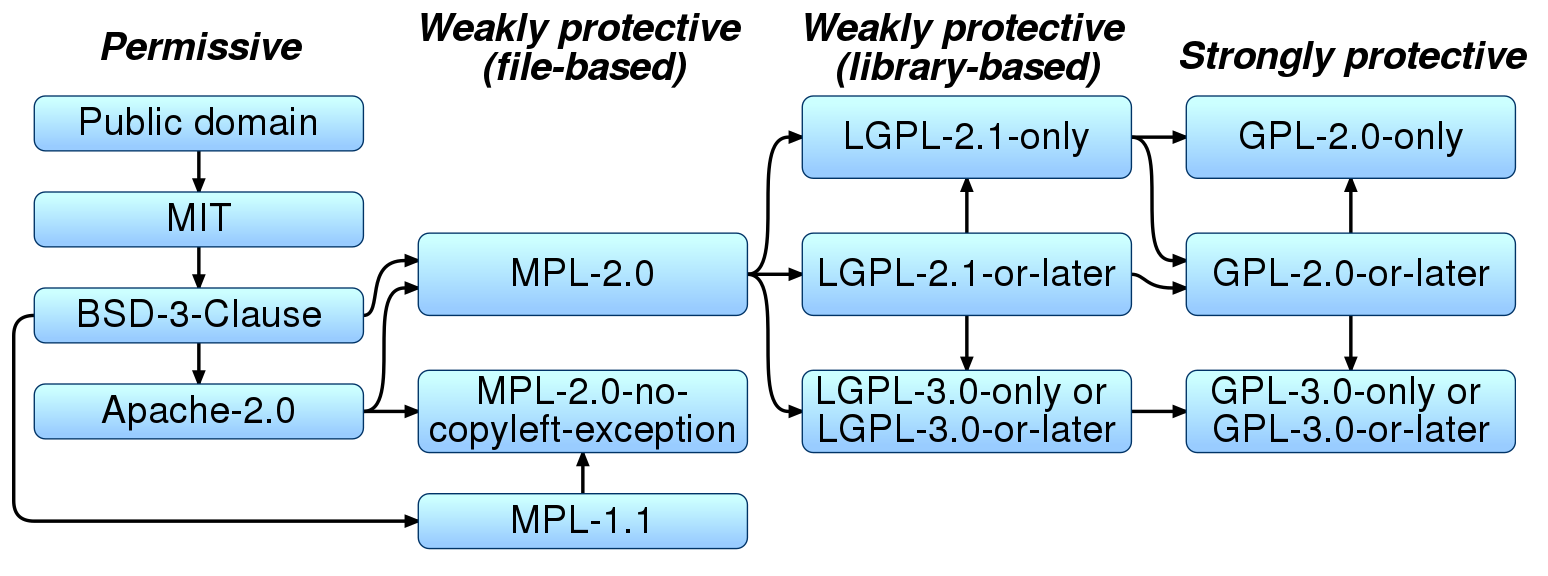
\includegraphics[width=\textwidth]{img/diagramas/licencias_compatibilidad.png}
    \caption{Compatibilidad de licencias.} \label{licencias_compatibilidad}
\end{figure}

En resumen estamos empleando la licencia GPL3~\cite{manual:GPL3} y CC-BY-SA-3.0~\cite{wiki:CreativeCommons}.

\begin{longtable}[c]{@{}ll@{}}
\toprule
\multicolumn{1}{c}{\textbf{Recurso}} & \multicolumn{1}{c}{\textbf{Licencia}} \\* \midrule
\endfirsthead
%
\endhead
%
\bottomrule
\endfoot
%
\endlastfoot
%
Código Fuente & GPL3 \\
Documentación & CC-BY-SA-3.0 \\
Imágenes & CC-BY-SA-3.0 \\* \bottomrule \\
%Vídeos & CC-BY-SA-3.0 \\* \bottomrule \\
\caption{Licencias aplicadas en el proyecto.}
\label{tab:licproy}\\
\end{longtable}

\begin{figure}[h]
  \begin{subfigure}
    
\includegraphics[width=0.3\textwidth]{img/herramientas/licencia_GPL3.png}
  \end{subfigure}
  \hfill
  \begin{subfigure}
    
\includegraphics[width=0.3\textwidth]{img/herramientas/licencia_cc.png}
  \end{subfigure}
\end{figure}

\apendice{Especificación de Requisitos}

\section{Introducción}

Una muestra de cómo podría ser una tabla de casos de uso:

% Caso de Uso 1 -> Consultar Experimentos.
\begin{table}[p]
	\centering
	\begin{tabularx}{\linewidth}{ p{0.21\columnwidth} p{0.71\columnwidth} }
		\toprule
		\textbf{CU-1}    & \textbf{Ejemplo de caso de uso}\\
		\toprule
		\textbf{Versión}              & 1.0    \\
		\textbf{Autor}                & Alumno \\
		\textbf{Requisitos asociados} & RF-xx, RF-xx \\
		\textbf{Descripción}          & La descripción del CU \\
		\textbf{Precondición}         & Precondiciones (podría haber más de una) \\
		\textbf{Acciones}             &
		\begin{enumerate}
			\def\labelenumi{\arabic{enumi}.}
			\tightlist
			\item Pasos del CU
			\item Pasos del CU (añadir tantos como sean necesarios)
		\end{enumerate}\\
		\textbf{Postcondición}        & Postcondiciones (podría haber más de una) \\
		\textbf{Excepciones}          & Excepciones \\
		\textbf{Importancia}          & Alta o Media o Baja... \\
		\bottomrule
	\end{tabularx}
	\caption{CU-1 Nombre del caso de uso.}
\end{table}

\section{Objetivos generales}

\section{Catálogo de requisitos}

\section{Especificación de requisitos}



%\apendice{Especificación de diseño}

\section{Introducción}

\section{Diseño de datos}

\section{Diseño procedimental}

\section{Diseño arquitectónico}



\apendice{Documentación técnica de programación}

\section{Introducción}

\section{Estructura de directorios}

\section{Manual del programador}

\section{Compilación, instalación y ejecución del proyecto}

\section{Pruebas del sistema}

\apendice{Documentación de usuario}

\section{Introducción}

%Se recomienda a los usuarios seguir cuidadosamente cada sección de este manual para garantizar una implementación exitosa y para aprovechar todas las capacidades que ofrece el sistema IoT de monitorización de invernaderos. 
Este documento está diseñado para facilitar la comprensión y el uso del sistema, contribuyendo así a una experiencia de usuario satisfactoria y a la consecución de los objetivos de monitorización de cultivos de cannabis medicinal de manera eficaz y económica.

%\section{Requisitos de usuarios}

\section{Instalación Física}
Se tiene que instalar el firmware en la Raspberry Pi Pico W para que podamos programarlo mediante Micropython.
Primero descargamos el firmware de Micropython desde su página oficial~\cite{misc:MicropythonFirmware}.

Para fines prácticos nombraremos al firmware descargado: \textbf{rp2-pico.uf2}.

\begin{figure}[h]
\centering
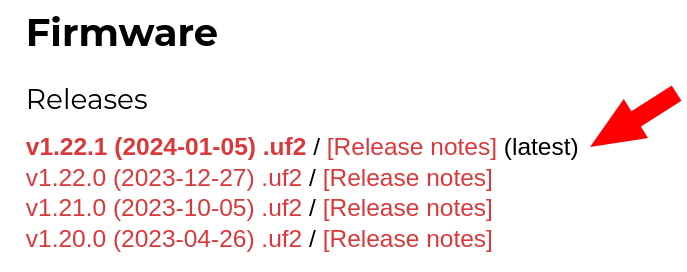
\includegraphics[width=0.7\textwidth]{img/herramientas/micropython_firmware.png}
\caption{Descargar el firmware más reciente.}
\end{figure}

Conectar el puerto usb de la Raspberry Pi Pico W manteniendo presionado el botón \textbf{BOOTSEL}.

\begin{figure}[h]
\centering
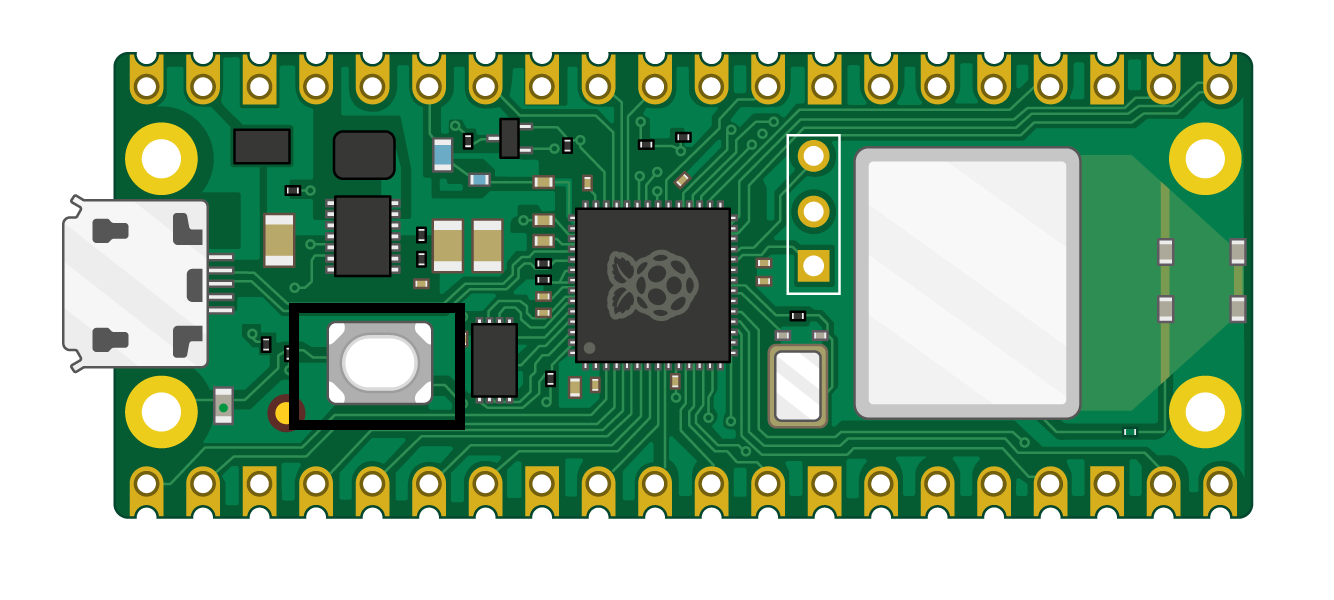
\includegraphics[width=1\textwidth]{img/herramientas/rpipicow_boton.png}
\caption{Conectar usb manteniendo presionado.}
\end{figure}

Se ha creado un script en bash al que llamamos \textbf{instaladorFirmware.sh}. La ejecución de este permitirá instalar el firmware de Micropython en la Raspberry Pi Pico W.


\begin{lstlisting}[language=sh, firstnumber=0, basicstyle=\normalsize, caption={Script en bash para instalar el firmware Micropython.}] 
puerto=$(sudo dmesg | tail | grep -o 'sd[b-z]1')
sudo mkdir /mnt/pico
sudo mount /dev/$puerto /mnt/pico
sudo cp rp2-pico.uf2 /mnt/pico
sudo sync
\end{lstlisting}

Tener presente que el archivo \textbf{instaladorFirmware.sh} y el firmware descargado, deben estar en el mismo directorio.

\begin{lstlisting}[language=sh, firstnumber=0, basicstyle=\normalsize, caption={Comando para dar permisos de ejecución.}] 
sudo chmod +x instaladorFirmware.sh\end{lstlisting}

\begin{lstlisting}[language=sh, firstnumber=0, basicstyle=\normalsize, caption={Comando para ejecutar el instalador de Firmware.}] 
sudo ./instaladorFirmware.sh\end{lstlisting}


Usando el IDE Thonny~\cite{misc:Thonny} y con Micropython vamos a poder programar el hardware. Lo podemos descargar e instalar desde su pagina oficial~\cite{misc:Thonny}.

Tenemos que hacer unas configuraciones simples antes de poder usar el IDE Thonny con Micropython en nuestra Raspberry Pi Pico W.

Hacemos clic en \textbf{Run/Configure interpreter}.

\begin{figure}[h]
	\centering
	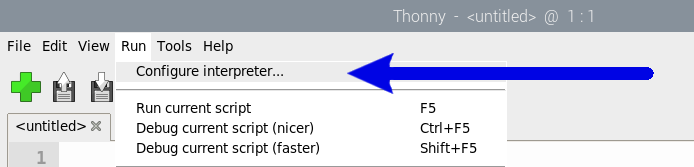
\includegraphics[width=0.9\textwidth]{img/desarrollo/thonny_interpreter.png}
	\caption{Abrimos el configurador del interpreter.}
\end{figure}

Seleccionamos que usaremos \textbf{Micropython} para Raspberry Pi Pico y seleccionamos el puerto que corresponde su conexión por usb.

\begin{figure}[h]
	\centering
	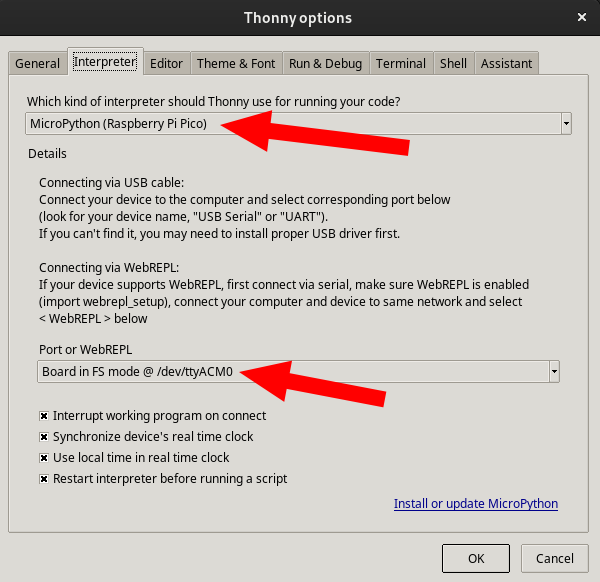
\includegraphics[width=0.9\textwidth]{img/desarrollo/thonny_seleccionInterpreter.png}
	\caption{Habilitamos Thonny para Micropython.}
\end{figure}

Usar los archivos del directorio \textbf{Hardware} para guardarlos en la Raspberry Pi Pico W usando el IDE Thonny.

\begin{figure}[h]
	\centering
	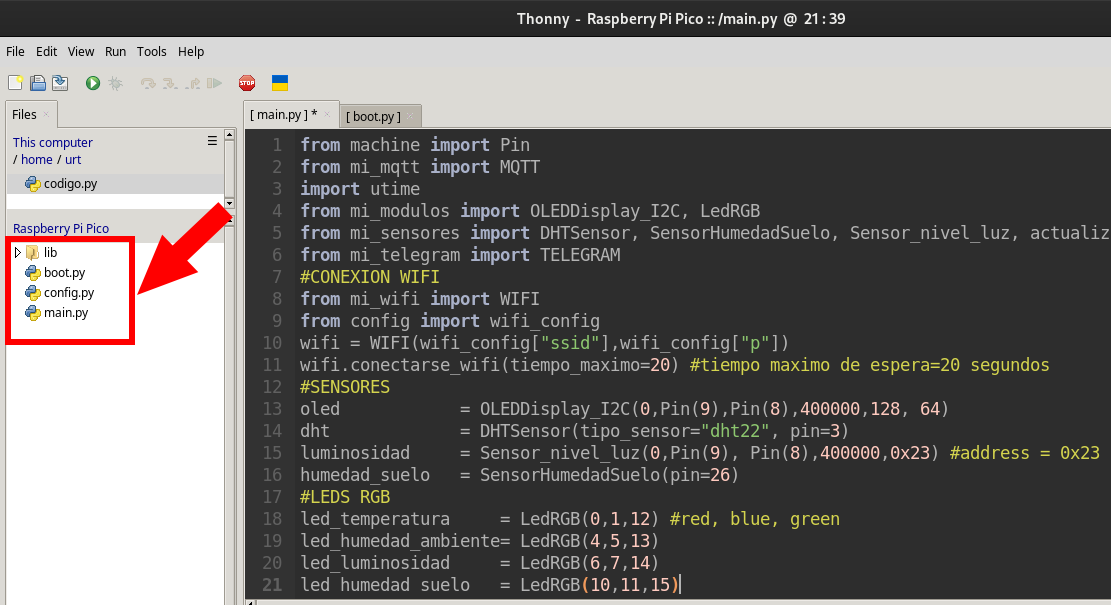
\includegraphics[width=0.9\textwidth]{img/desarrollo/thonny_archivosNecesarios.png}
	\caption{Archivos necesarios para ejecutar en el hardware.}
\end{figure}


\begin{figure}[h]
	\centering
	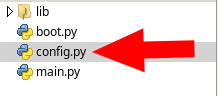
\includegraphics[width=0.4\textwidth]{img/desarrollo/thonny_config.png}
	\caption{Archivo de configuración en Micropython.}
\end{figure}

Modificamos el archivo \textbf{config.py} con nuestras credenciales.

\begin{lstlisting}[language=sh, firstnumber=0, basicstyle=\normalsize, caption={Configurar SSID y clave wifi.}] 
wifi_config = {
    'ssid':'SSID_WIFI',
    'p':'TU_PASSWORD_WIFI'
}\end{lstlisting}



\begin{lstlisting}[language=sh, firstnumber=0, basicstyle=\normalsize, caption={Configución de bot de Telegram.}] 
utelegram_config = {
    'token': 'BOT_TOKEN_TELEGRAM',
    'chat_id': 'BOT_CHAT_ID'
}
\end{lstlisting}

\begin{lstlisting}[language=sh, firstnumber=0, basicstyle=\normalsize, caption={Configuración de umbrales para los sensores.}] 
umbrales_sensores = {
    'TEMPERATURA_MINIMA': 30,
    'HUMEDAD_MINIMA': 30,
    'LUMINOSIDAD_MINIMA': 30,
    'HUMEDAD_SUELO_MINIMA': 20,
    'TEMPERATURA_MAXIMA': 35,
    'HUMEDAD_MAXIMA': 70,
    'LUMINOSIDAD_MAXIMA': 150,
    'HUMEDAD_SUELO_MAXIMA': 80
}
\end{lstlisting}

\begin{lstlisting}[language=sh, firstnumber=0, basicstyle=\normalsize, caption={Configuración MQTT.}] 
mqtt_config = {
    'server': '1.39.4.38', #IP DE TU SERVIDOR LAMP
    'port': 1883, #PUERTO USADO POR MQTT
    'topic_pub': 'invernadero/sensores',
    'topic_sub': 'invernadero/ordenes',
    'topic_umb': 'invernadero/umbrales',
    'client_id_pub': 'TFG_UBU_mqtt_id_pub',
    'client_id_sub': 'TFG_UBU_mqtt_id_sub',
    'client_id_umb': 'TFG_UBU_mqtt_id_umb'
}
\end{lstlisting}

\begin{lstlisting}[language=sh, firstnumber=0, basicstyle=\normalsize, caption={Configuración Wlan para usar ip fija.}] 
wlan_config = {
    'ip':'192.168.1.232',
    'mask':'255.255.255.0',
    'gateway':'192.168.1.1',
    'dns':'8.8.8.8' 
}
\end{lstlisting}

Una vez que haz completado las credenciales ya puedes desconectar y volver a conectar la Rapsberry Pi Pico W, al arrancar automáticamente se ejecutará la programación ya establecida.

Solo volverás a usar el IDE Thonny si quieres cambiar algo en el código o en el archivo de configuración.

Ahora procedemos a hacer las conexiones en el hardware.

Solo comprobar que todas las conexiones sean coherentes a la imagen.

\begin{figure}[h]
\centering
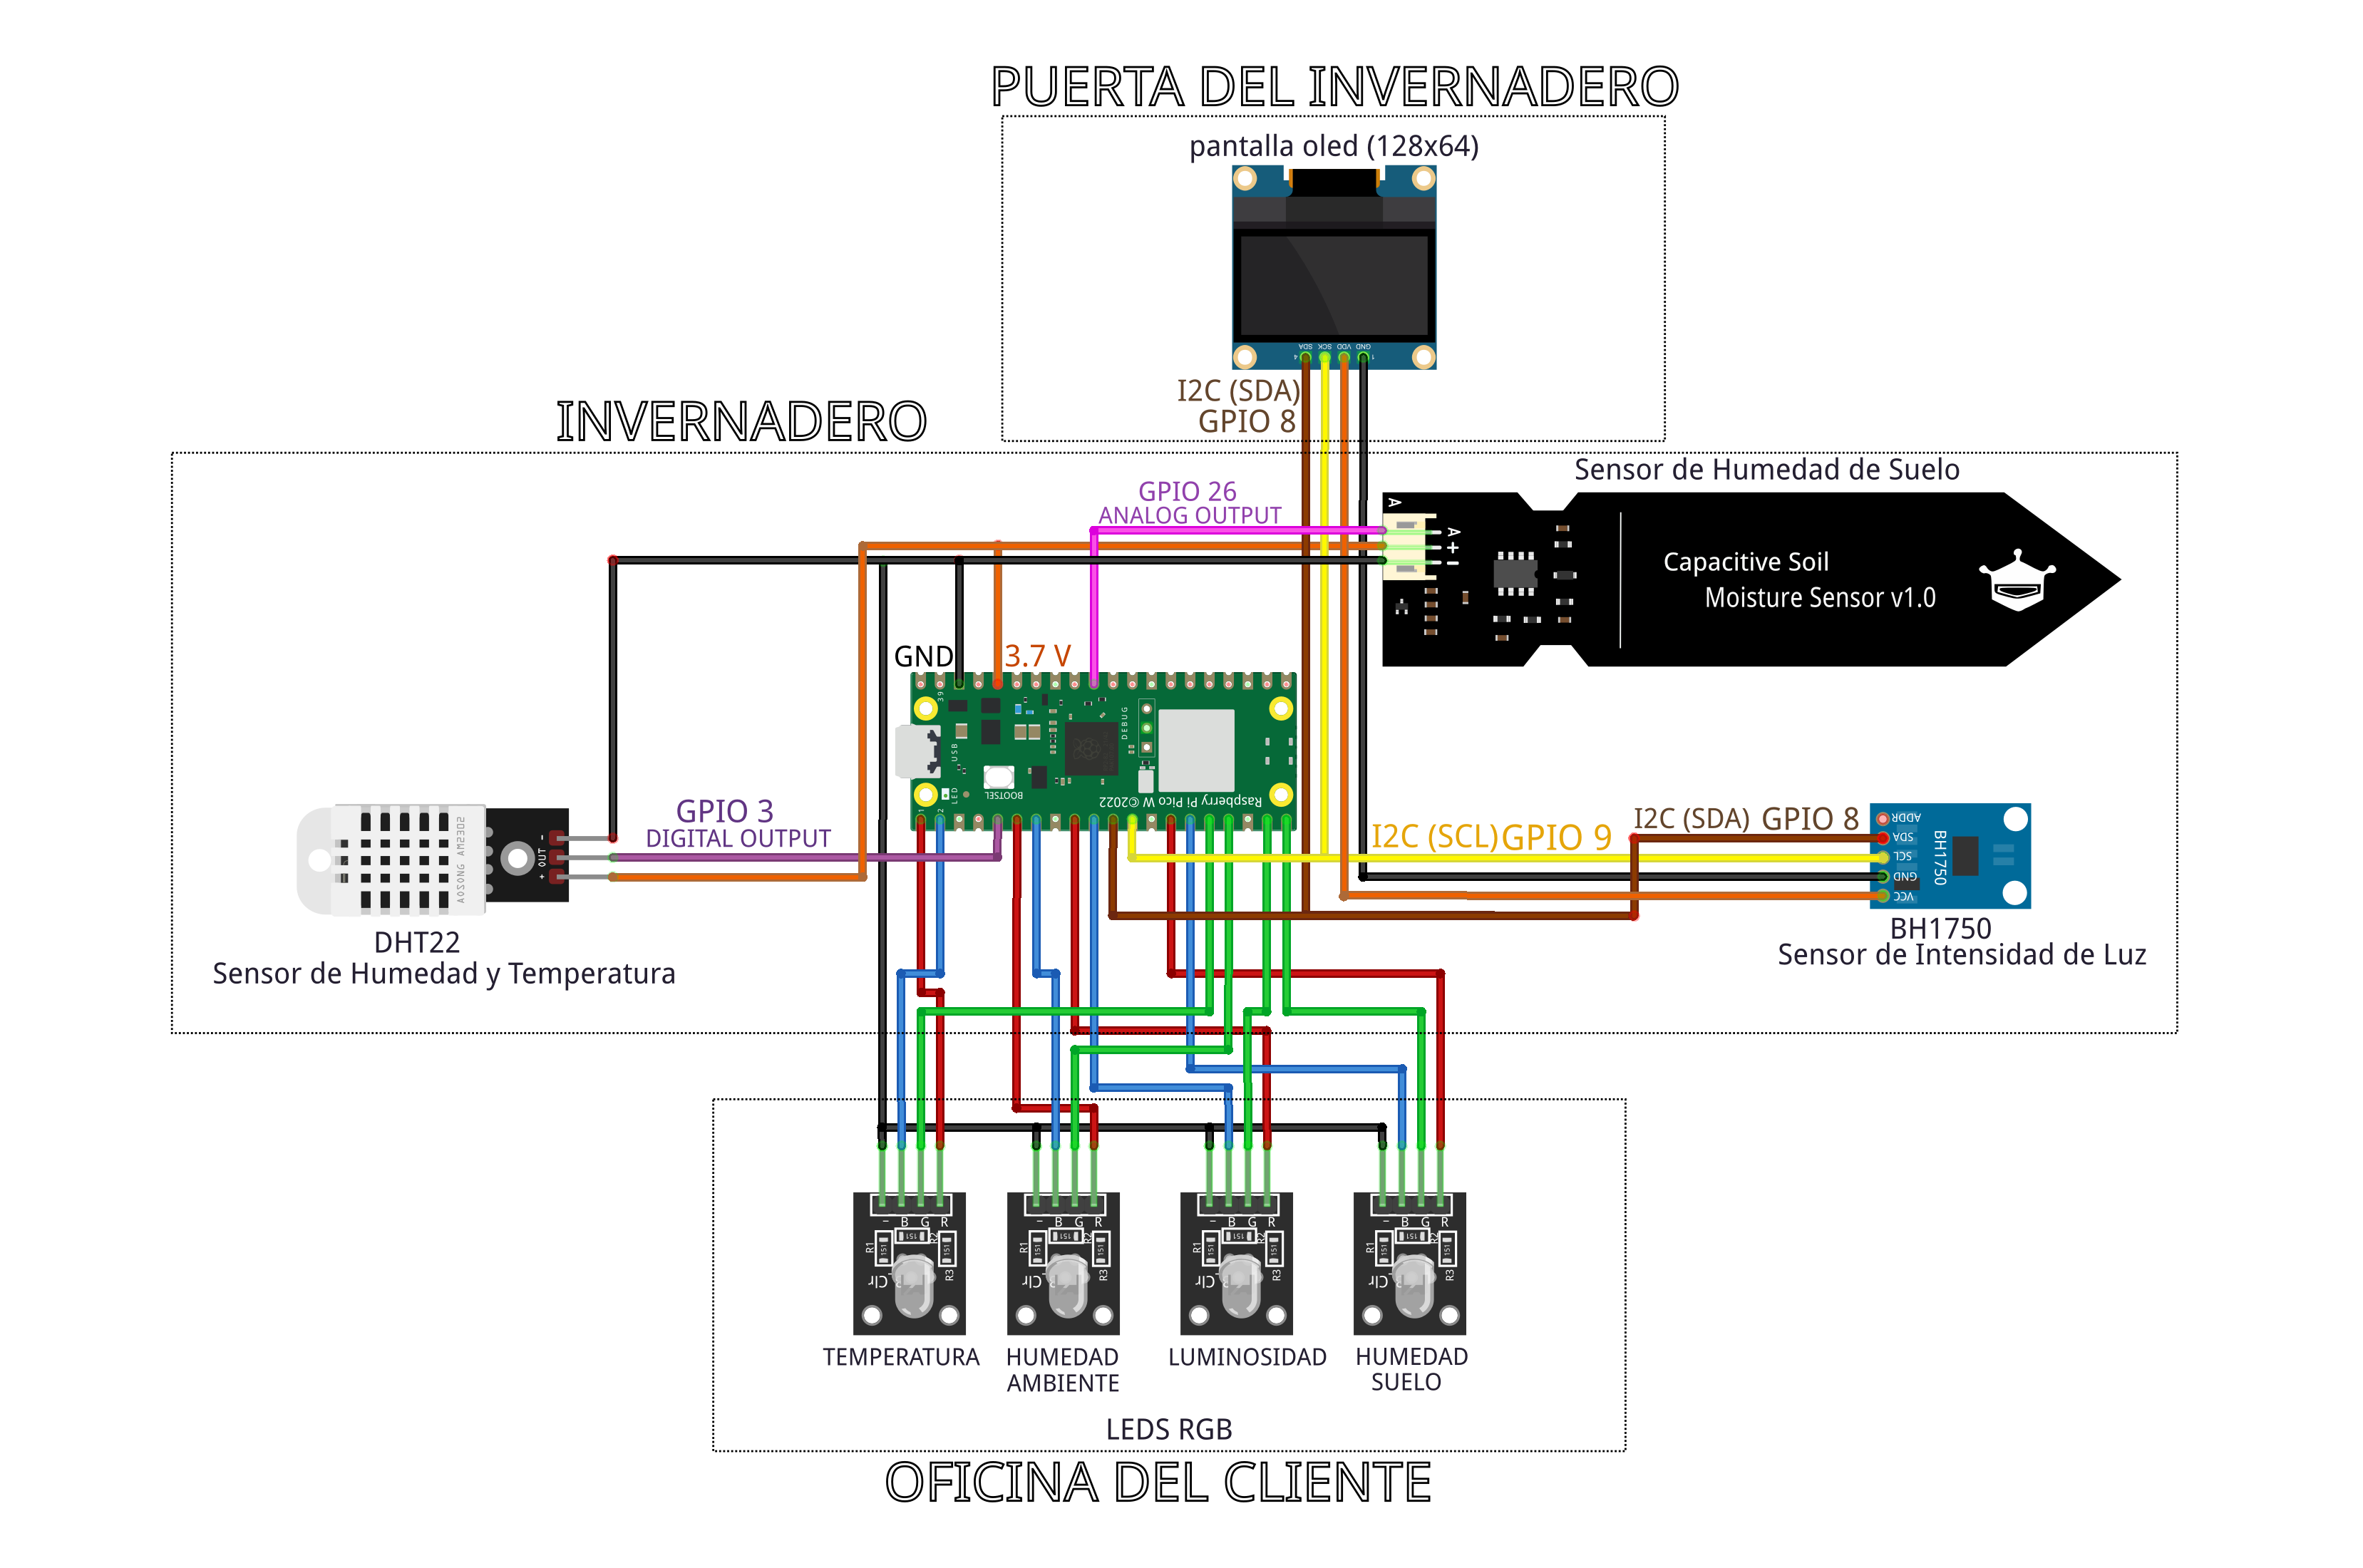
\includegraphics[width=1\textwidth]{img/diagramas/conexiones.png}
\caption{Conexiones del hardware para el cliente.}
\end{figure}


\section{Instalación del software}

\subsection{Servidor LAMP}
Se ha creado un script en bash para hacer las instalaciones automáticamente al que se ha nombrado \textbf{InstaladorServidor.sh}.

\begin{lstlisting}[language=sh, firstnumber=0, basicstyle=\normalsize, caption={Damos permisos de ejecución a \textbf{InstaladorServidor.sh}.}] 
sudo chmod +x InstaladorServidor.sh
\end{lstlisting}

\begin{lstlisting}[language=sh, firstnumber=0, basicstyle=\normalsize, caption={Contenido de \textbf{InstaladorServidor.sh}.}] 
sudo apt install apache2
sudo apt install mysql-server
sudo apt install php
sudo apt install ssh
sudo apt install phpmyadmin
sudo apt install vsftpd
sudo apt install ufw 
sudo apt install nodejs
sudo apt install pm2
sudo apt install npm
sudo apt install express
sudo apt install mosquitto 
\end{lstlisting}

\begin{lstlisting}[language=sh, firstnumber=0, basicstyle=\normalsize, caption={Ejecutamos \textbf{InstaladorServidor.sh}.}] 
sudo ./InstaladorServidor.sh
\end{lstlisting}

\subsection{Creación de base de datos}
\begin{lstlisting}[language=sh, firstnumber=0, basicstyle=\normalsize, caption={Comando para acceder a Mysql.}] 
sudo mysql\end{lstlisting}

\begin{lstlisting}[language=sh, firstnumber=0, basicstyle=\normalsize, caption={Comandos Mysql para crear Database \textbf{TFG\_UBU}.}] 
CREATE DATABASE TFG_UBU;
CREATE USER 'joseluis'@'%' IDENTIFIED BY 'Mipassword';
GRANT ALL ON TFG_UBU.* TO 'joseluis'@'%';
use TFG_UBU;
\end{lstlisting}


\begin{lstlisting}[language=sh, firstnumber=0, basicstyle=\normalsize, caption={Comandos Mysql para crear tabla \textbf{umbrales}.}] 
CREATE TABLE `umbrales` (
  `temperatura_minima` float NOT NULL,
  `temperatura_maxima` float NOT NULL,
  `humedad_ambiente_minima` float NOT NULL,
  `humedad_ambiente_maxima` float NOT NULL,
  `luminosidad_minima` float NOT NULL,
  `luminosidad_maxima` float NOT NULL,
  `humedad_suelo_minima` float NOT NULL,
  `humedad_suelo_maxima` float NOT NULL,
  `fecha_actualizacion` timestamp 
  NULL DEFAULT CURRENT_TIMESTAMP 
  ON UPDATE CURRENT_TIMESTAMP
) ENGINE=InnoDB DEFAULT CHARSET=utf8mb4;
INSERT INTO `umbrales` (
`temperatura_minima`, `temperatura_maxima`, 
`humedad_ambiente_minima`, `humedad_ambiente_maxima`, 
`luminosidad_minima`, `luminosidad_maxima`, 
`humedad_suelo_minima`, `humedad_suelo_maxima`) VALUES
(30, 35, 30, 70, 30, 150, 20, 80);
\end{lstlisting}

\begin{lstlisting}[language=sh, firstnumber=0, basicstyle=\normalsize, caption={Comandos Mysql para crear tabla \textbf{sensores}.}] 
CREATE TABLE `sensores` (
  `id` int NOT NULL AUTO_INCREMENT,
  `fecha` date DEFAULT NULL,
  `hora` time DEFAULT NULL,
  `temperatura` decimal(4,2) DEFAULT NULL,
  `humedad` decimal(4,2) DEFAULT NULL,
  `intensidad_luz` decimal(4,2) DEFAULT NULL,
  `humedad_suelo` decimal(4,2) DEFAULT NULL,
  PRIMARY KEY (`id`)
) ENGINE=InnoDB DEFAULT CHARSET=utf8mb4;
\end{lstlisting}


\subsection{dashboard}

\begin{lstlisting}[language=sh, firstnumber=0, basicstyle=\normalsize, caption={Instalaciones necesarias.}] 
npm install express
npm install socket.io
\end{lstlisting}

Respecto al archivo \textbf{servers.js} debemos configurar respecto a la base de datos creada en el servidor LAMP:

\begin{lstlisting}[language=cpp, firstnumber=0, basicstyle=\normalsize, caption={Configuración de base de datos.}] 
const dbConfig = {
    host: 'localhost',
    port: 3307, // Puerto especificado aquí
    user: 'joseluis',
    password: 'TuPassword',
    database: 'TFG_UBU'
};
\end{lstlisting}

Solo se ejecuta una vez y siempre va a estar ejecutándose, incluso si se reinicia el servidor.

\begin{lstlisting}[language=sh, firstnumber=0, basicstyle=\normalsize, caption={Ejecución.}] 
mp2 start servers.js --name "dashboard"
\end{lstlisting}

\subsection{InverIoT}
Solo ejecutar el instalador \textbf{Instalador - InverIoT - v2.2.exe}.

\section{Manual del usuario}

Una vez todo está instalado y configurado ya puedes interactuar con las diferentes partes del proyecto.

\subsection{Hardware}
Solo conectar la Raspberry Pi Pico a una fuente de energía y está operativo.

\begin{figure}[h]
\centering
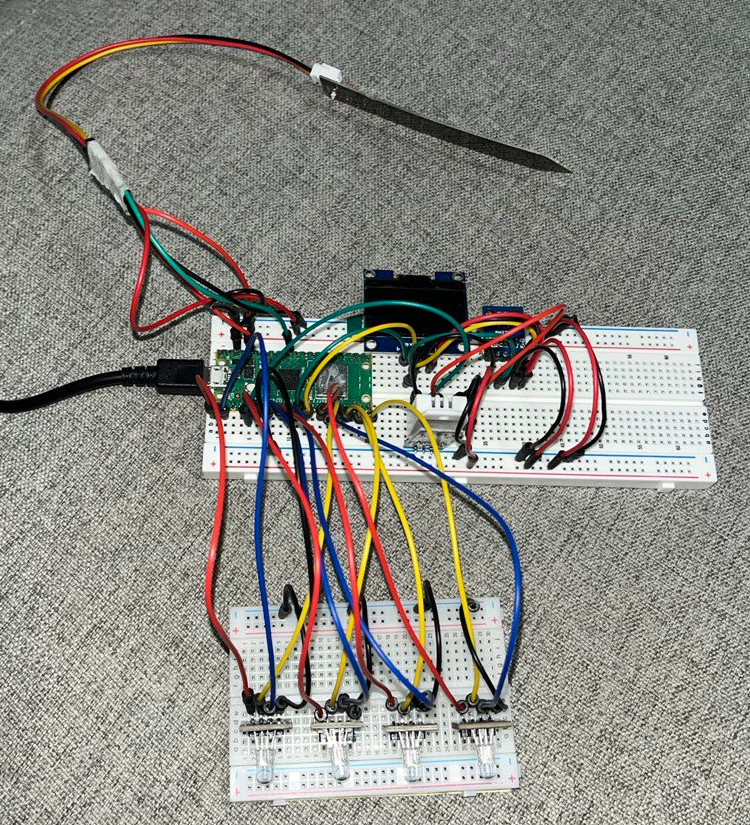
\includegraphics[width=0.9\textwidth]{img/fotos/conexiones_real.png}
\caption{Foto real de las conexiones.}
\end{figure}

Clavar el sensor de humedad de suelo en el punto que se desea monitorear.

\begin{figure}[h]
\centering
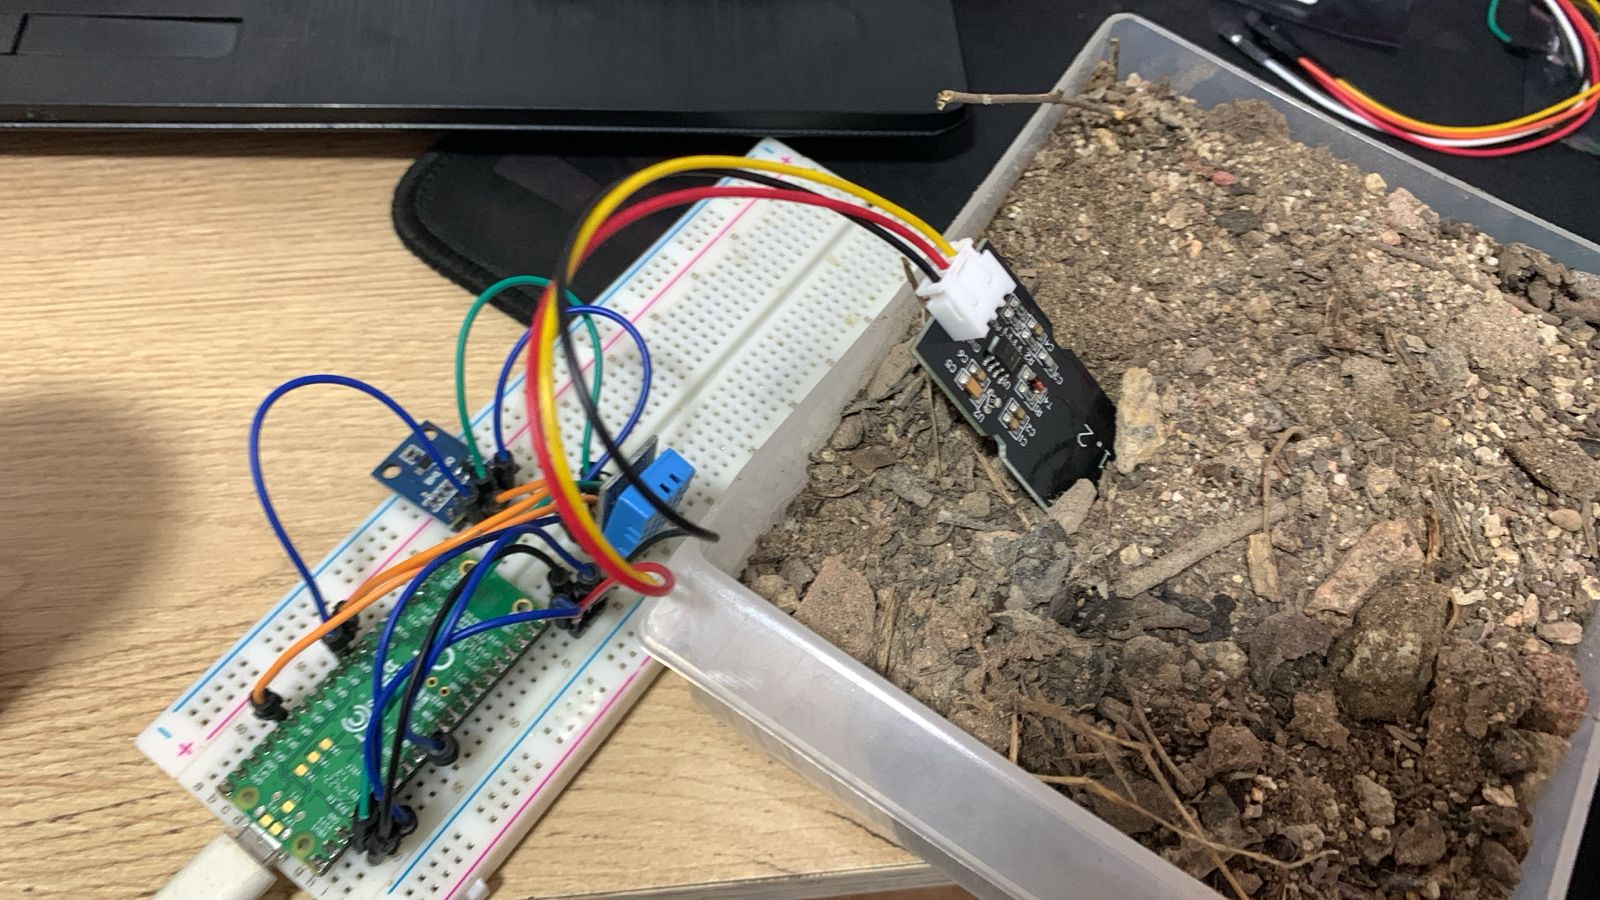
\includegraphics[width=0.7\textwidth]{img/fotos/sensorHumedadSuelo.png}
\caption{Sensor de humedad de suelo operativo.}
\end{figure}

Los valores en tiempo real se pueden ver en la pantalla oled con sus respectivas unidades.

\begin{figure}[h]
\centering
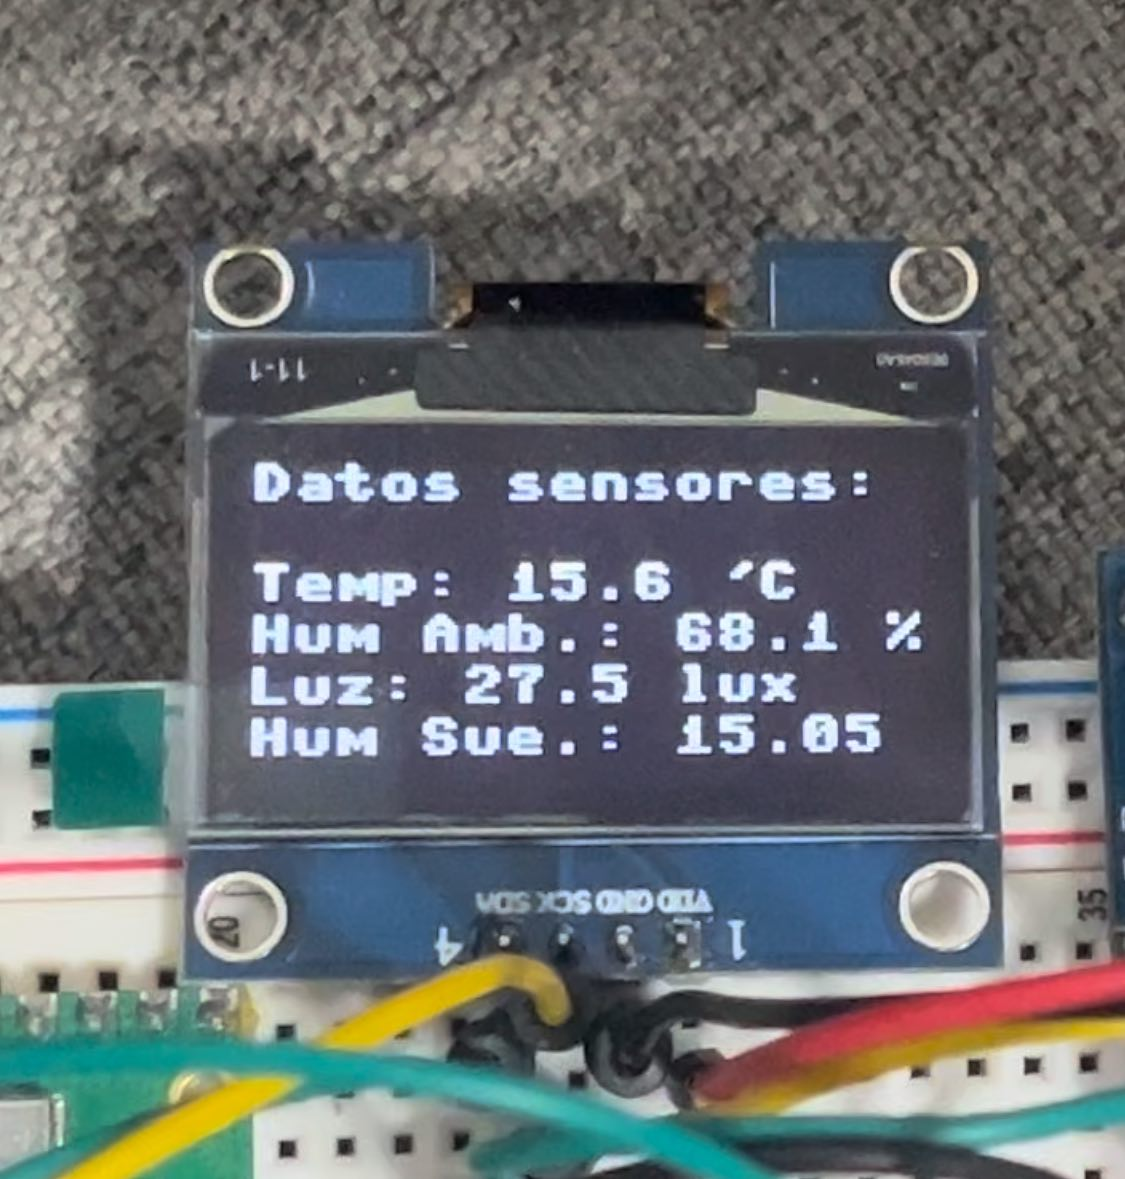
\includegraphics[width=0.71\textwidth]{img/fotos/oled1.png}
\caption{Pantalla oled mostrando los datos.}
\end{figure}

\subsection{InverIoT}

\begin{figure}[h]
\centering
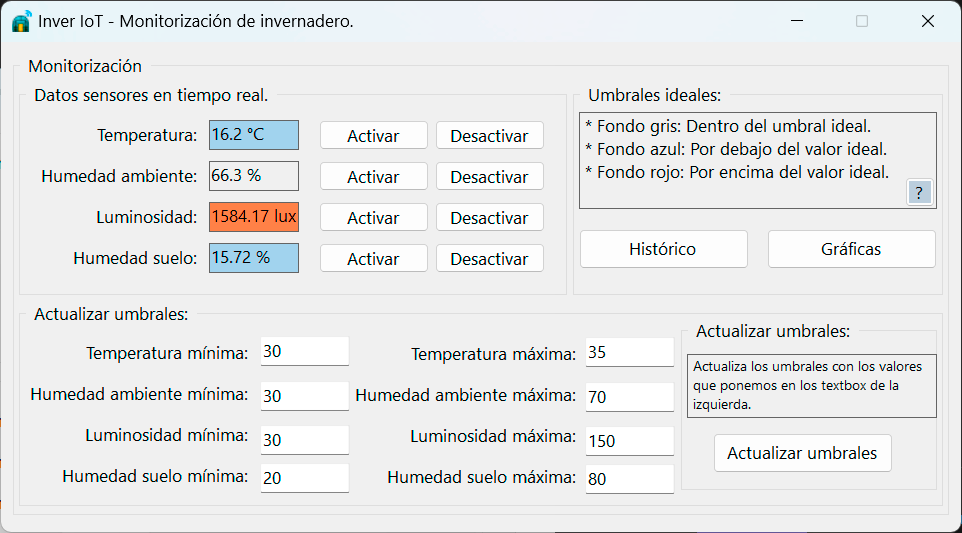
\includegraphics[width=1\textwidth]{img/desarrollo/InverIoT_Desktop.png}
\caption{Interfaz de la aplicación de escritorio.}
\end{figure}

La interfaz permite modificar los umbrales, tiene una comunicación bidireccional con la base de datos.

\begin{figure}[h]
\centering
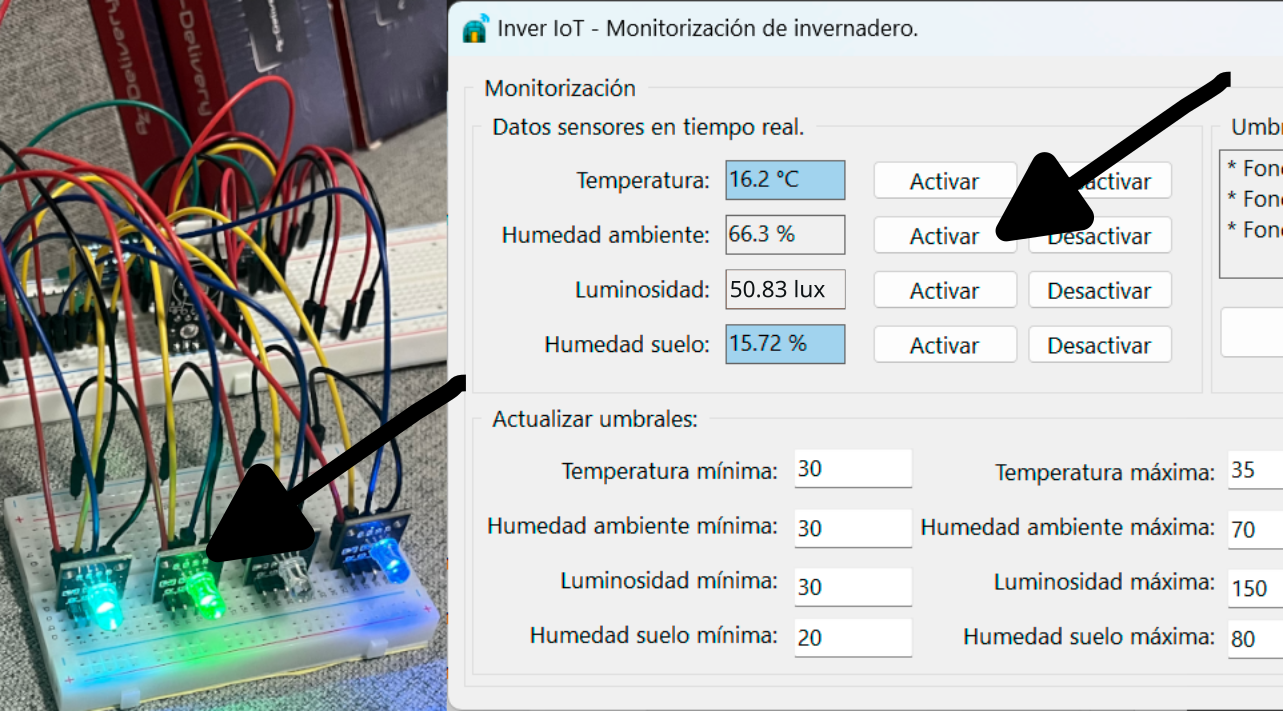
\includegraphics[width=1\textwidth]{img/desarrollo/InverIoT_verde_clickMecanismo.png}
\caption{Activación de mecanismo con un clic.}
\end{figure}

La activación del mecanismo está representado por el led verde prendido, pero si se desea activar otro mecanismo, solo desconectar del módulo led RGB el cable asociado al color verde, y conectarlo al mecanismo que se desea. Hacer esto solo si el nuevo mecanismo a activar es compatible en cuanto al voltaje necesario.


\begin{figure}[h]
\centering
\includegraphics[width=0.9\textwidth]{img/desarrollo/InverIoT_Histórico.png}
\caption{Accesso al histórico de datos.}
\end{figure}

\begin{figure}[h]
\centering
\includegraphics[width=1\textwidth]{img/desarrollo/InverIoT_Gráficas.png}
\caption{Capacidad de mostrar gráficas en un rango de fechas.}
\end{figure}

\subsection{dashboard}
Solo permite visualizar los datos, no envía comandos.

\begin{figure}[h]
\centering
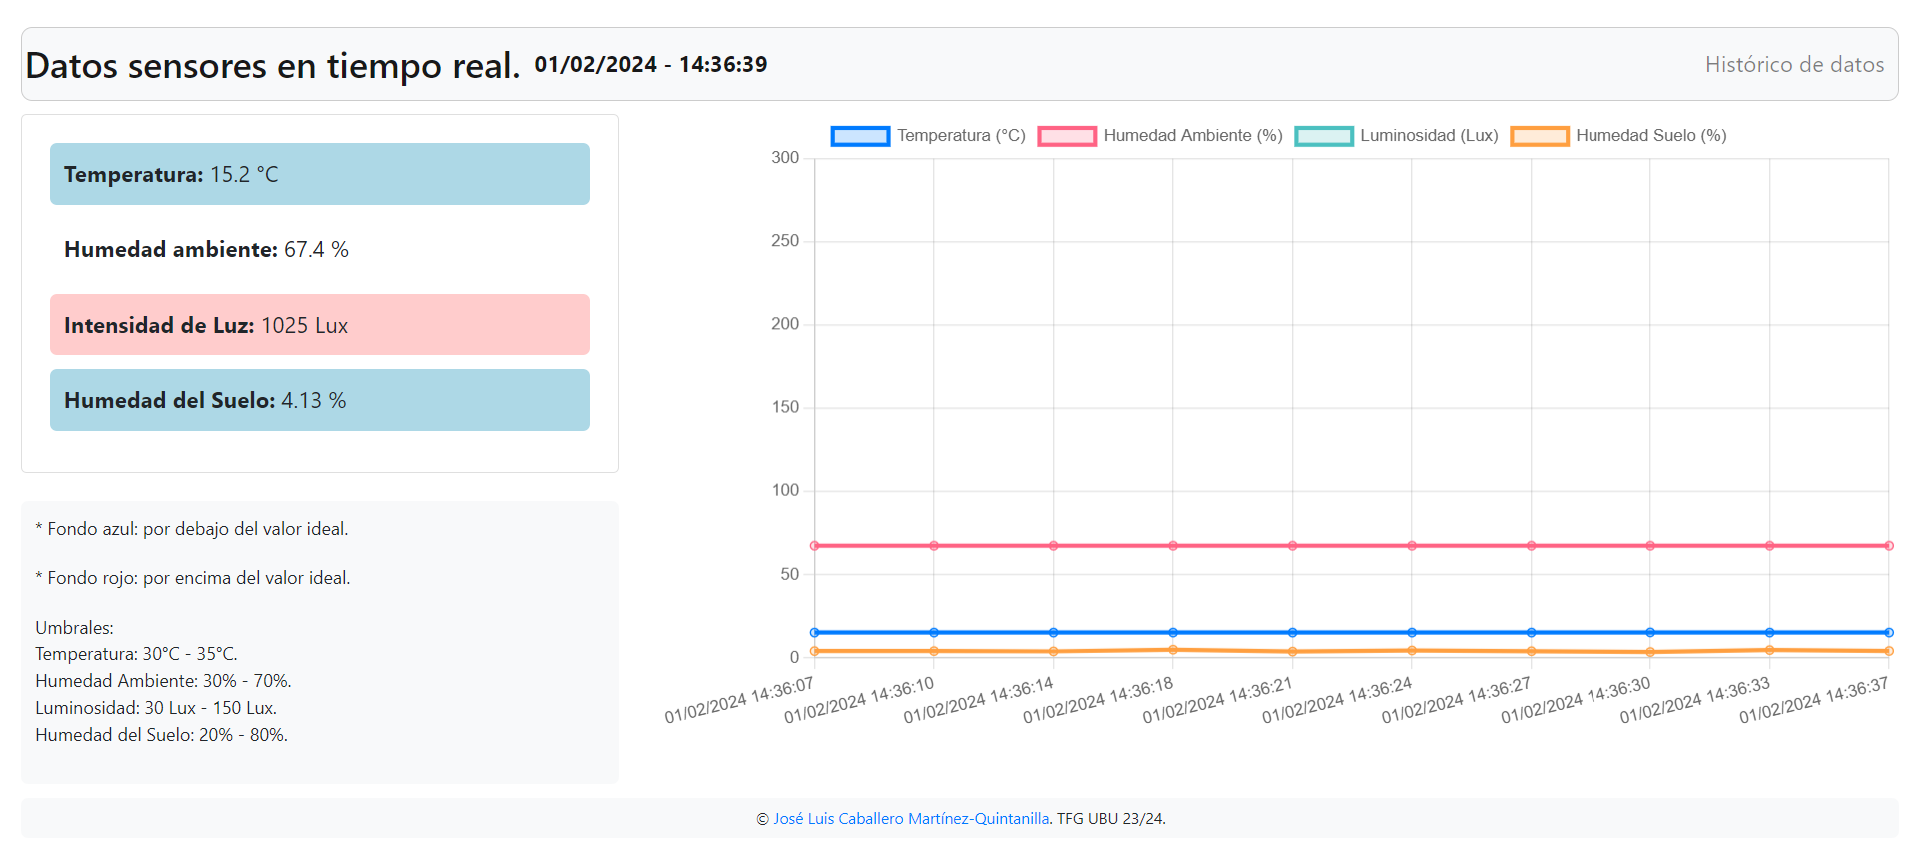
\includegraphics[width=1\textwidth]{img/desarrollo/Dashboard1.png}
\caption{El color rojo indica se ha sobrepasado el umbral.}
\end{figure}

\begin{figure}[h]
\centering
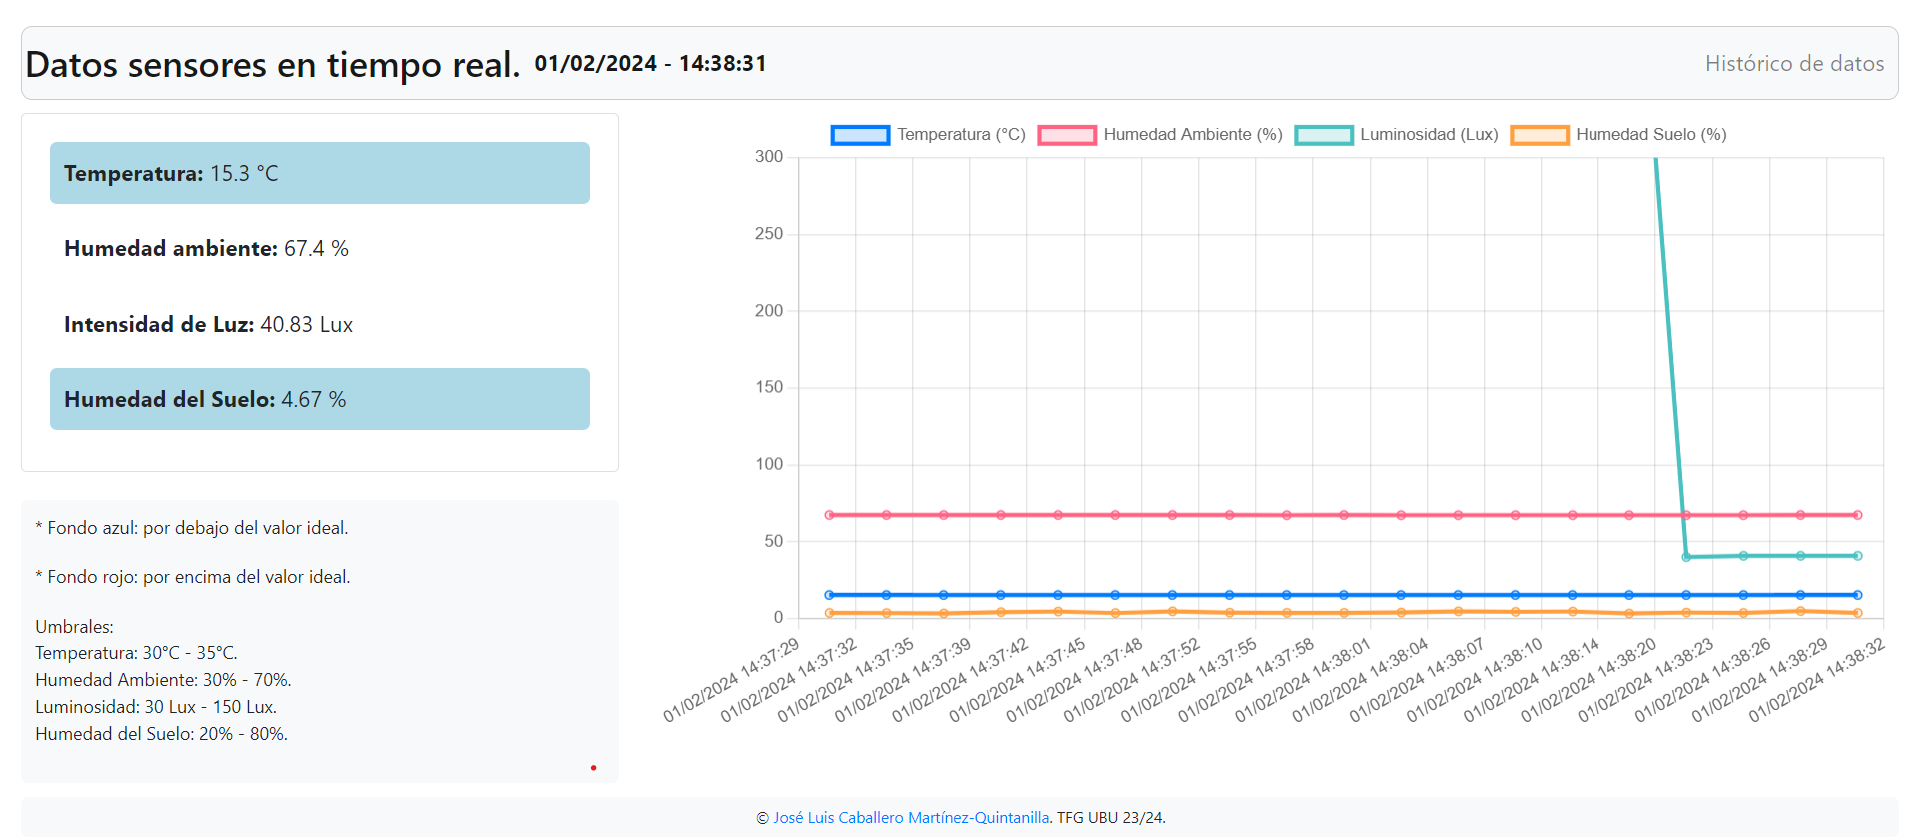
\includegraphics[width=1\textwidth]{img/desarrollo/Dashboard2.png}
\caption{El color azul indica está por debajo del umbral.}
\end{figure}

\subsection{Bot de telegram}
Permite enviar comandos y recibir alertas.

\begin{figure}[h]
\centering
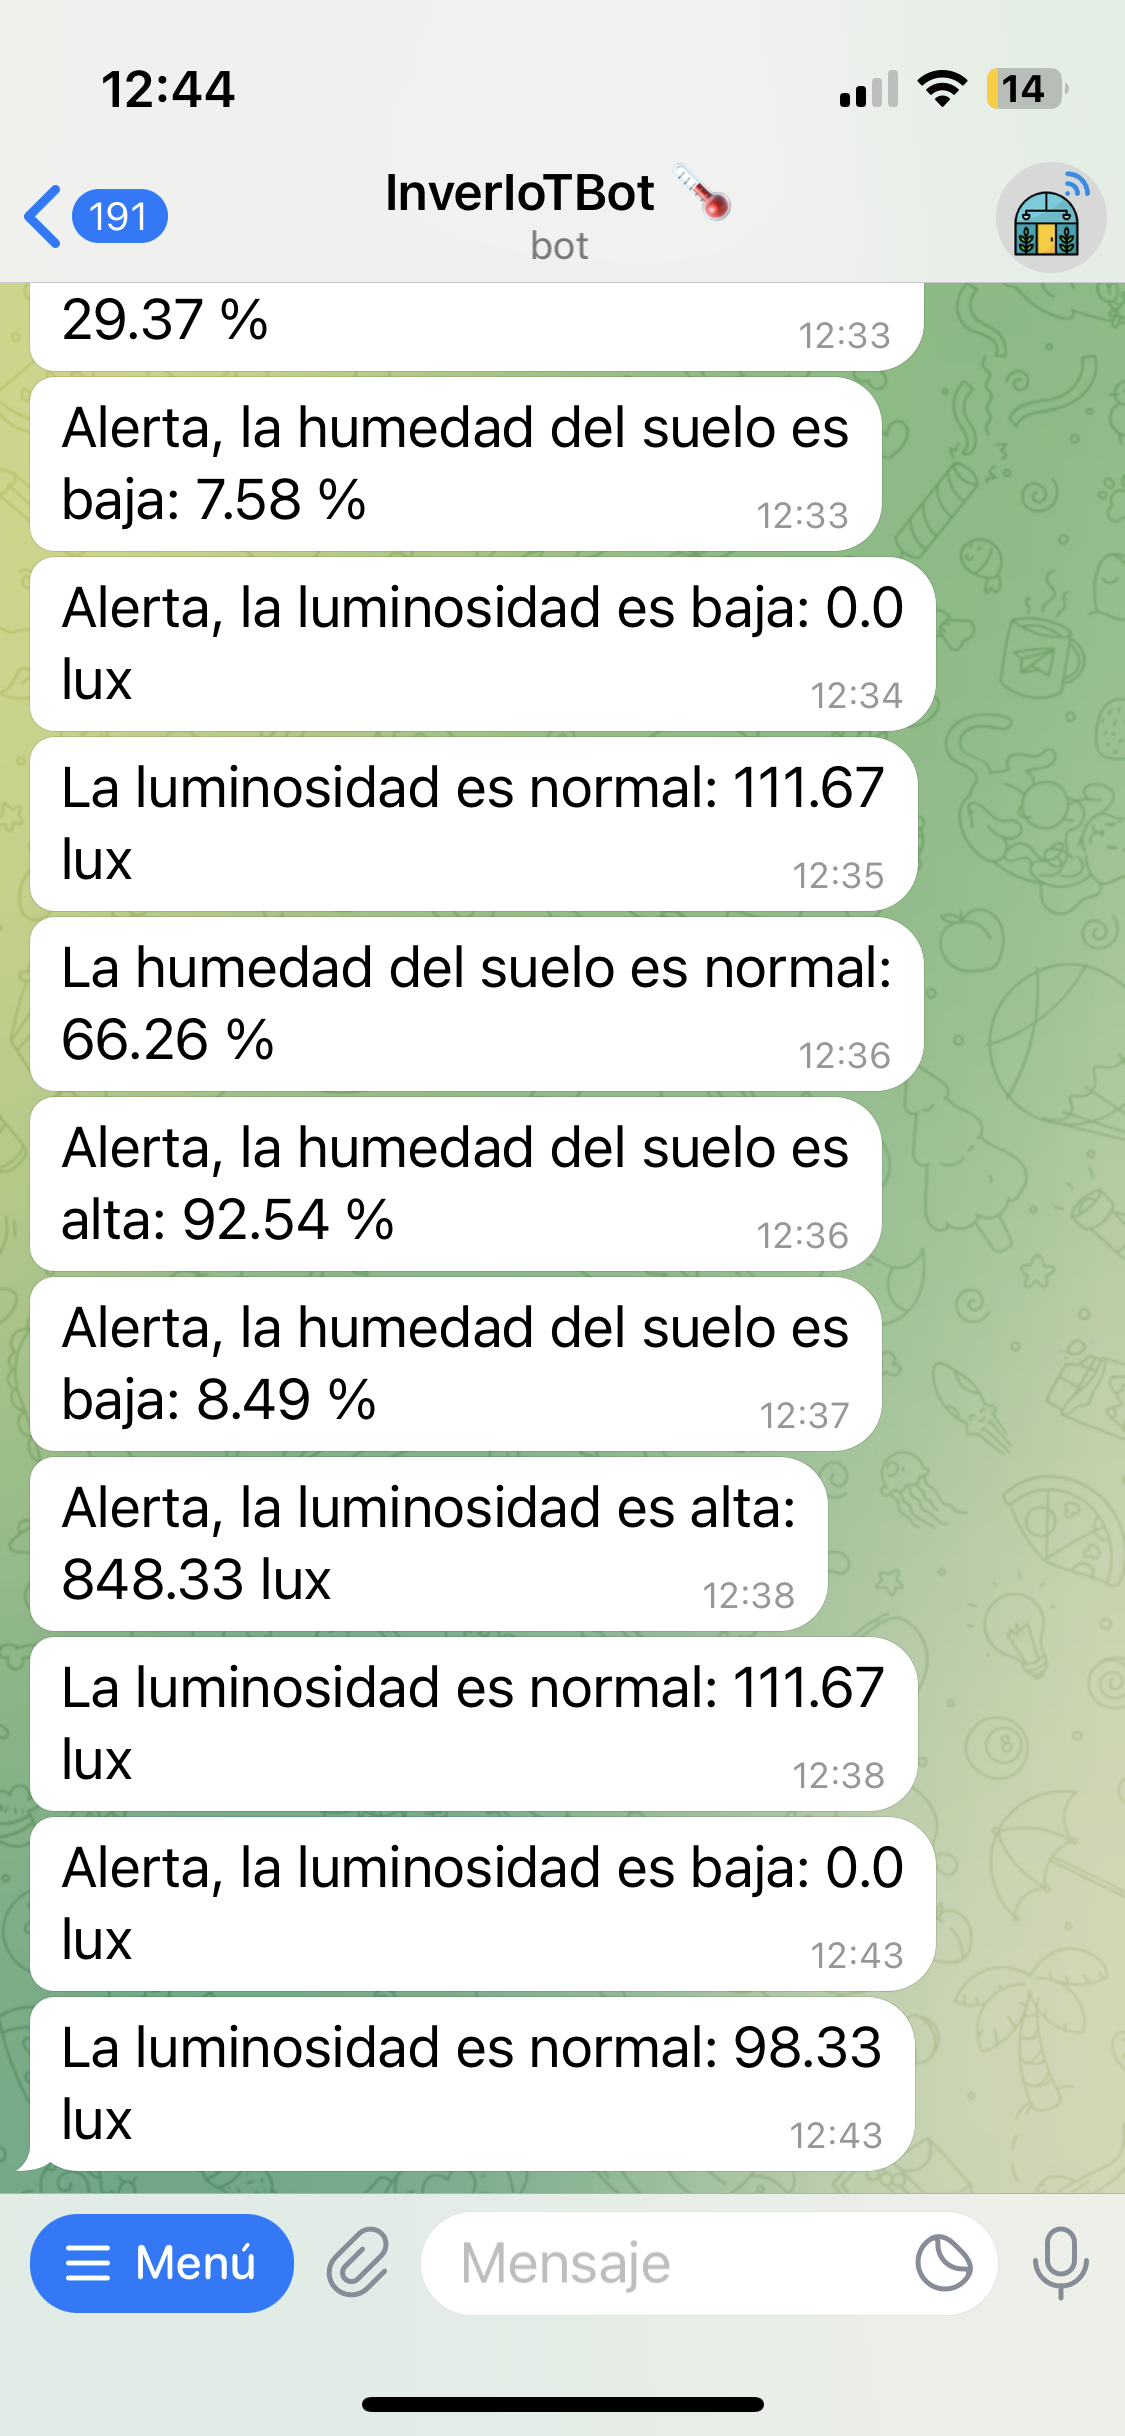
\includegraphics[width=0.7\textwidth]{img/desarrollo/BotTelegram_alertas.png}
\caption{Alertas recibidas por el bot de Telegram.}
\end{figure}

\begin{figure}[h]
\centering
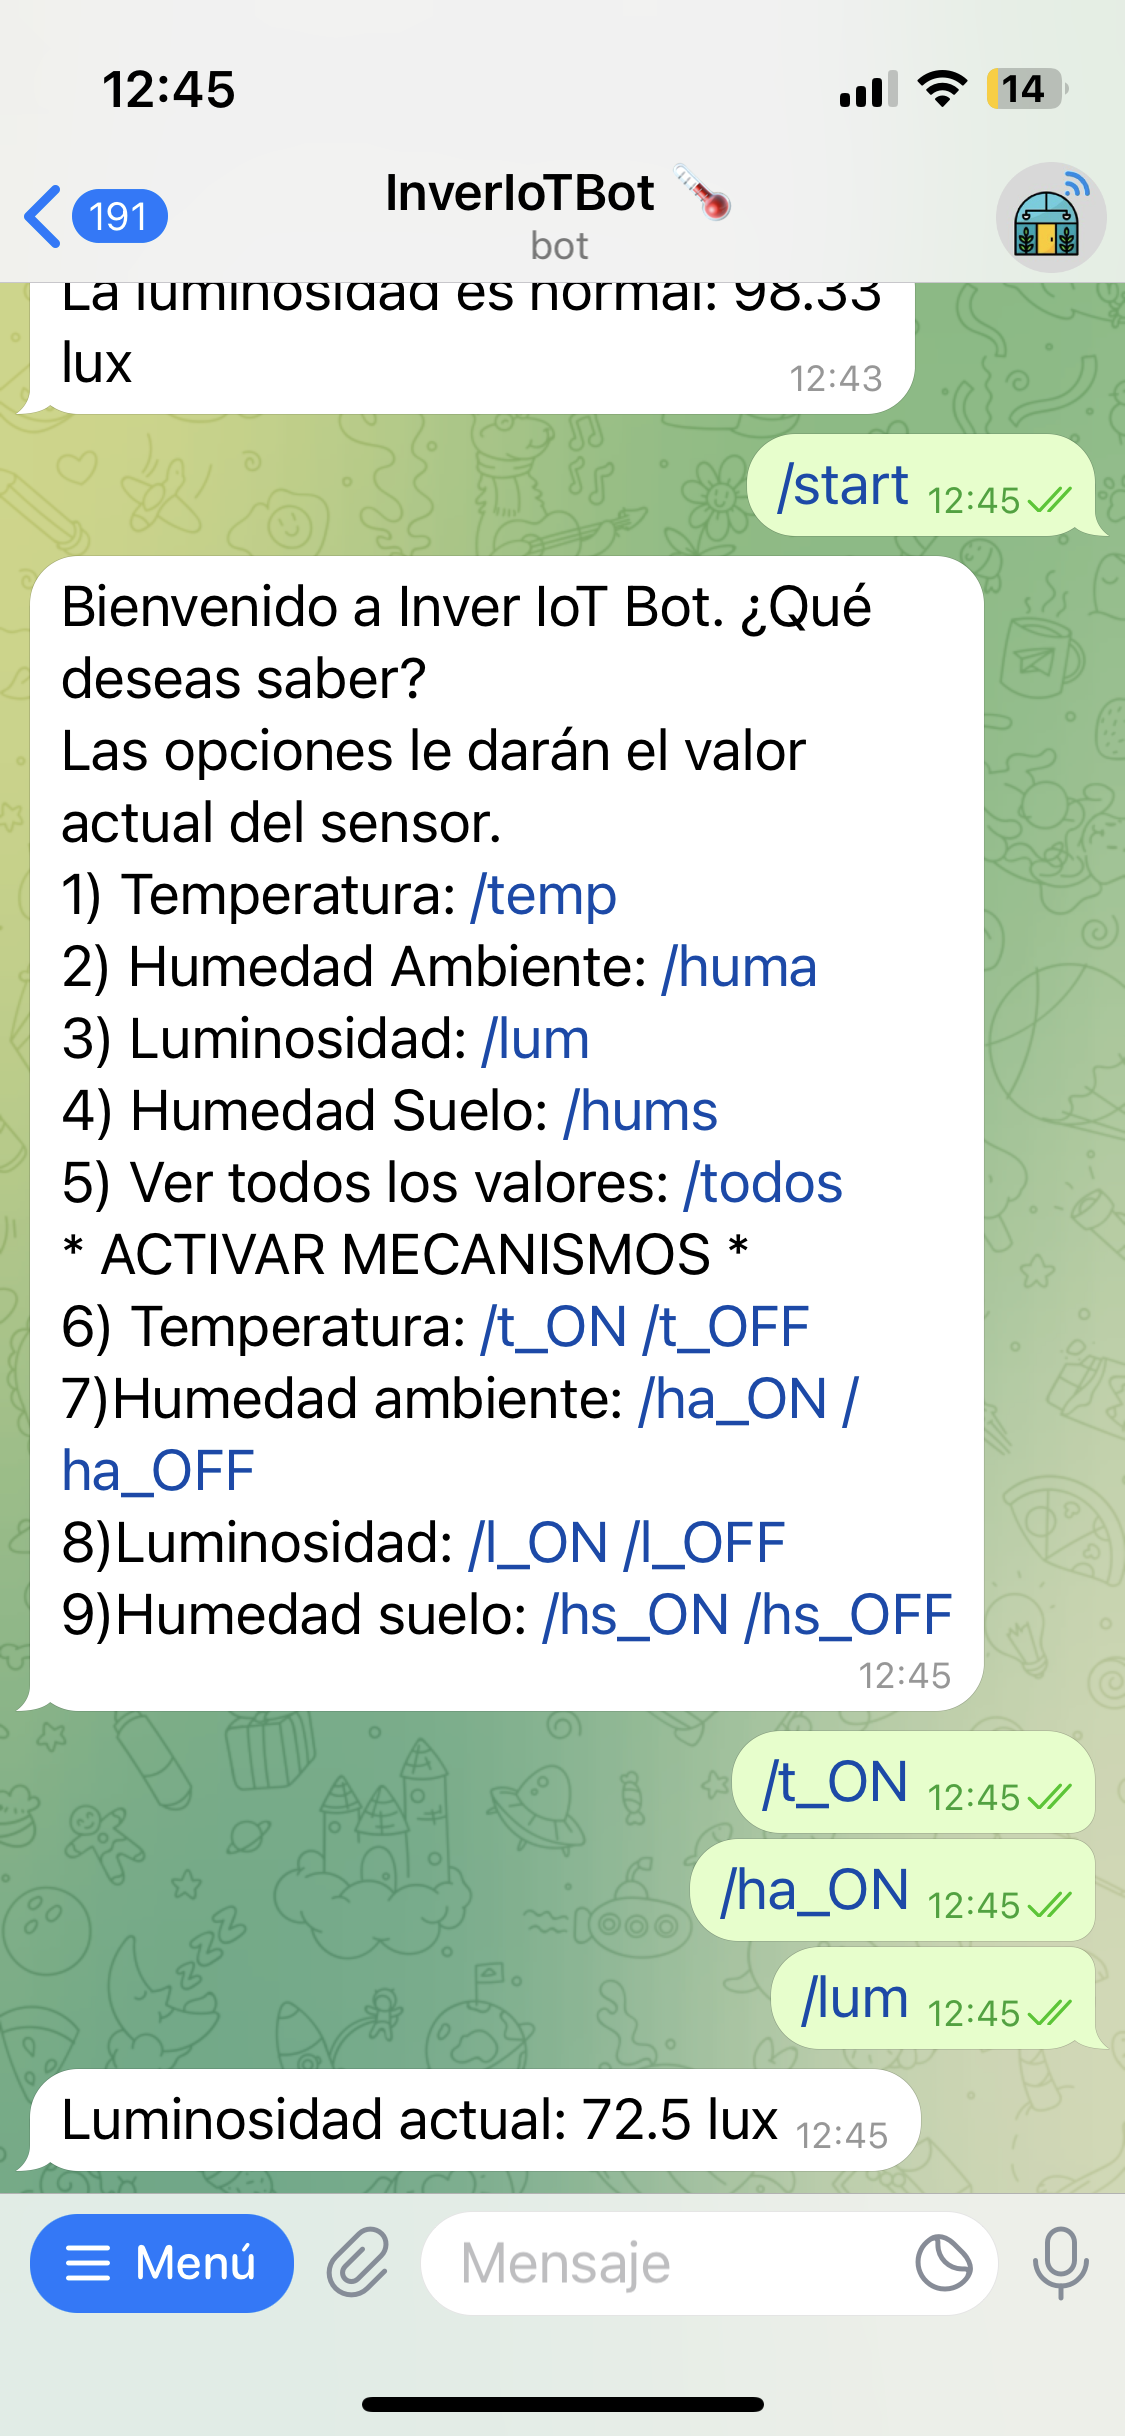
\includegraphics[width=0.7\textwidth]{img/desarrollo/BotTelegram_comandos.png}
\caption{Capacidad de enviar comandos desde Telegram.}
\end{figure}

%\apendice{Anexo de sostenibilización curricular}

\section{Introducción}
Este anexo incluirá una reflexión personal del alumnado sobre los aspectos de la sostenibilidad que se abordan en el trabajo.
Se pueden incluir tantas subsecciones como sean necesarias con la intención de explicar las competencias de sostenibilidad adquiridas durante el alumnado y aplicadas al Trabajo de Fin de Grado.

Más información en el documento de la CRUE \url{https://www.crue.org/wp-content/uploads/2020/02/Directrices_Sosteniblidad_Crue2012.pdf}.

Este anexo tendrá una extensión comprendida entre 600 y 800 palabras.



\bibliographystyle{plain}
\bibliography{bibliografiaAnexos}

\end{document}
